\PassOptionsToPackage{table}{xcolor}   % house style: striped tables (extras.tex)
%%%%%%%%%%%%%%%%%%%%%%%%%%%%%%%%%%%%%%%%%
% Macro Regime–Based Asset Rotation
% Two-column academic journal style
% Modeled after the uploaded LaTeX article template
%%%%%%%%%%%%%%%%%%%%%%%%%%%%%%%%%%%%%%%%%

\documentclass[10pt, a4paper, twocolumn]{article}

% ─── Packages ───────────────────────────────────────
\usepackage[utf8]{inputenc}
\usepackage[T1]{fontenc}
\usepackage{mathpazo}                       % Palatino font (matches template)
\usepackage{microtype}                      % Better typography
\usepackage[english]{babel}
\usepackage{amsmath,amssymb,amsfonts}
\usepackage{graphicx}
\usepackage{booktabs}
\usepackage{tabularx}
\usepackage{float}
\usepackage{caption}
\usepackage{subcaption}
\usepackage[colorlinks=true,linkcolor=blue,citecolor=blue,urlcolor=blue]{hyperref}
\usepackage[numbers,sort&compress]{natbib}
\usepackage{fancyhdr}
\usepackage{geometry}
\usepackage{enumitem}
\usepackage{xcolor}
\usepackage{titlesec}
\usepackage{abstract}
\usepackage{etoolbox}
\usepackage{multirow}
\usepackage{array}
\usepackage{makecell}

% ─── Page geometry (matches template) ──────────────
\geometry{
  top=2.0cm,
  bottom=2.0cm,
  left=1.8cm,
  right=1.8cm,
  columnsep=0.8cm
}

% ─── Header / footer (journal style like template) ─
\pagestyle{fancy}
\fancyhf{}
\renewcommand{\headrulewidth}{0.4pt}
\fancyhead[L]{\small\textit{Forced Flows at the Index Close}}
\fancyhead[R]{\small\textit{QUANTT Research}}
\fancyfoot[L]{\small\textit{Queen's University Algorithmic \& Network Trading Team (2026)}}
\fancyfoot[R]{\small\thepage}

% ─── Section formatting (centered, matches template) ──
\titleformat{\section}
  {\large\bfseries\centering}{\thesection.}{0.5em}{}
\titleformat{\subsection}
  {\normalsize\bfseries}{\thesubsection}{0.5em}{}
\titleformat{\subsubsection}
  {\normalsize\bfseries\itshape}{\thesubsubsection}{0.5em}{}

% ─── Abstract formatting ─────────────────────────────
\renewcommand{\abstractnamefont}{\normalfont\bfseries}
\renewcommand{\abstracttextfont}{\normalfont\small\itshape}

% ─── Float spacing (tighten gaps around tables/figures) ──
\setlength{\textfloatsep}{8pt plus 2pt minus 2pt}
\setlength{\intextsep}{8pt plus 2pt minus 2pt}
\setlength{\floatsep}{8pt plus 2pt minus 2pt}
\setlength{\abovecaptionskip}{4pt}
\setlength{\belowcaptionskip}{2pt}

% ─── Custom commands ──────────────────────────────────
\newcommand{\shratio}{\text{Sharpe}}
\newcommand{\regime}[1]{\textsc{#1}}

%═══════════════════════════════════════════════════════
% ─── House additions (load right after preamble.tex, before \begin{document}) ───
% Needs \PassOptionsToPackage{table}{xcolor} as the FIRST line of the .tex file (before \documentclass).
% Navy accent on headings, captions and table rules; striped tables; a key-findings box.
\usepackage{colortbl}
\usepackage[most]{tcolorbox}
\definecolor{qnavy}{HTML}{1B365D}
\definecolor{qblue}{HTML}{4A7AB5}
\definecolor{qstripe}{HTML}{F2F5FA}
\definecolor{qbox}{HTML}{EEF2F8}

\titleformat{\section}{\large\bfseries\centering\color{qnavy}}{\thesection.}{0.5em}{}
\titleformat{\subsection}{\normalsize\bfseries\color{qnavy}}{\thesubsection}{0.5em}{}
\titleformat{\subsubsection}{\normalsize\bfseries\itshape\color{qnavy}}{\thesubsubsection}{0.5em}{}

\captionsetup{font=small, labelfont={bf,color=qnavy}, labelsep=period}
\hypersetup{linkcolor=qblue, citecolor=qblue, urlcolor=qblue}

% Booktabs rules in navy; zebra rows with \qstripes before the tabular (inside the table float).
\makeatletter
\renewcommand{\toprule}{\arrayrulecolor{qnavy}\specialrule{\heavyrulewidth}{\abovetopsep}{\belowrulesep}\arrayrulecolor{black}}
\renewcommand{\bottomrule}{\arrayrulecolor{qnavy}\specialrule{\heavyrulewidth}{\aboverulesep}{\belowbottomsep}\arrayrulecolor{black}}
\makeatother
\newcommand{\qstripes}{\rowcolors{2}{qstripe}{white}}
\newcommand{\qhead}[1]{\textbf{\color{qnavy}#1}}

% Key findings: full width (put it inside the \twocolumn[{...}] title block after the abstract,
% or in a figure*). Usage: \begin{keyfindings} \item ... \end{keyfindings}
\newenvironment{keyfindings}
  {\begin{tcolorbox}[enhanced, colback=qbox, colframe=qnavy, boxrule=0pt, leftrule=2.5pt,
     arc=0pt, left=6pt, right=6pt, top=4pt, bottom=4pt, fontupper=\small,
     title={\small\bfseries Key findings}, coltitle=qnavy, colbacktitle=qbox, attach title to upper={\par\vspace{2pt}}]
   \begin{itemize}[nosep, leftmargin=*, label={\color{qnavy}\textbullet}]}
  {\end{itemize}\end{tcolorbox}}

% Source line under a figure or table: \qsource{CRSP via WRDS; author's calculations.}
\newcommand{\qsource}[1]{\par\vspace{1pt}{\footnotesize\color{black!60}\textit{Source:} #1}\par}
\newcommand{\mn}{\ensuremath{-}}
\newcolumntype{L}{>{\raggedright\arraybackslash}X}
\newcolumntype{R}{>{\raggedleft\arraybackslash}X}
\newcolumntype{P}[1]{>{\raggedright\arraybackslash}p{#1}}
\renewcommand{\arraystretch}{1.08}
% Float placement: allow up to two full-width floats at the top of a page so figures stay near their text.
\setcounter{dbltopnumber}{2}
\setcounter{topnumber}{3}
\setcounter{totalnumber}{5}
\renewcommand{\dbltopfraction}{0.82}
\renewcommand{\topfraction}{0.88}
\renewcommand{\textfraction}{0.08}
\renewcommand{\floatpagefraction}{0.75}
\renewcommand{\dblfloatpagefraction}{0.75}
% Do not favour column breaks before headings (with ragged bottoms this left gaps).
\makeatletter\@secpenalty=0\makeatother

\begin{document}
\raggedbottom

% ─── Title block ─────────────────────────────────────
\twocolumn[{%
\begin{center}
{\LARGE\bfseries Forced Flows at the Index Close:\\
Point-in-Time Event Studies of Index Rebalances\\ in Canada, Europe and the United States\par}
\vspace{0.8em}
{\large Simon Jarvis\par}
\vspace{0.4em}
{\normalsize
QUANTT --- Queen's University Algorithmic \& Network Trading Team\\
\vspace{0.3em}
}
\vspace{0.5em}

\begin{minipage}{0.92\textwidth}
\rule{\linewidth}{0.4pt}
\vspace{0.3em}
\textbf{Abstract}\\[0.3em]
\small\itshape
Index funds must trade every addition, deletion and weight change at the official close of the effective day, whatever the price. We measure what that obligation has been worth to other traders, and when, in four rule-based index families: the Russell US June reconstitution (2008--2025), the S\&P/TSX Composite (2006--2026), the STOXX Europe 600 (2008--2026) and the German DAX family (2008--2025), with MSCI Canada and MSCI Europe reviews (2018--2026) added for the close. For every review we rebuild the provider's ranking point in time six months out, three months out and on the ranking date, and hold the predicted changes, false positives included, against matched controls. The large moves in the names that were actually added or deleted (for additions, +21\% to +36\% against controls from six months out) are almost entirely selection on the ranking variable and cannot be captured. The capturable trade that paid before 2016 has largely gone: Russell predicted additions earned +6.7\% from end-December in 2008--2015 and $-$1.9\% in 2016--2025. Two pockets remain, gross of costs: S\&P/TSX additions predicted three months out (+3.4\% under the plain rules, +6.8\% with filters chosen after seeing the errors, 2016--2026) and small-cap DAX-family promotions (+3.1\% from six months out), which earn nothing once weighted by what can be deployed. On the trade day the close does not reliably move with index demand outside US deletions priced below \$5, reversals are mostly overnight, and the one liquid liquidity-supply trade found, in Russell up-migrants, earns +42 bp gross overnight. Larger predicted flow does not move the close more. Paper forecasts for the November and December 2026 reviews were logged with file hashes before the announcements; replays on mid-2026 reviews are reported but are not out of sample. All returns are gross of spreads, impact, taxes and borrow.
\vspace{0.3em}
\rule{\linewidth}{0.4pt}
\end{minipage}

\vspace{0.5em}
\begin{minipage}{0.92\textwidth}
\begin{keyfindings}
\item Names actually added rose 21--36\% against controls from six months out; the portfolios of \emph{predicted} changes earned between $-$2.4\% and +2.2\% over the same window. The pre-event run-up is selection, not a capturable premium.
\item The hold-to-the-close trade has decayed: Russell predicted additions earned +6.7\% from end-December in 2008--2015 ($t = 2.3$) and $-$1.9\% in 2016--2025.
\item Two pockets remain, gross of costs: S\&P/TSX additions predicted three months out (+3.4\% under the plain rules, $t = 2.4$, 2016--2026) and small-cap DAX-family promotions (+3.1\%, $t = 2.7$), which earn nothing once weighted by deployable size.
\item At the close, buying Russell up-migrants and selling at the next open earned +42 bp ($t = 4.3$, 17 of 18 reconstitutions); outside US stocks under \$5 the close does not move with index demand, and larger flow does not move it more.
\item Free-data forecasts of the June 2026 reviews were accurate at the cut-off (STOXX 600 additions 12 of 14) but weak seven weeks out (2 of 12 additions found); forecasts for the November and December 2026 reviews were logged with file hashes before the announcements.
\end{keyfindings}
\end{minipage}

\vspace{0.3em}
{\footnotesize \textbf{Date:} November 2026.}
\end{center}
\vspace{1em}
}]

%═══════════════════════════════════════════════════════
\section{Introduction}
\label{sec:intro}

An index fund must hold what its index holds. When a provider adds a stock, deletes one or changes a weight, a fund that tracks the index has to make the same change at the official closing price of the effective day, because that is the price the index itself uses. The fund's demand does not respond to price: it buys an addition and sells a deletion at whatever the closing auction prints. Other traders can be paid for meeting that demand in two broad ways. They can own future additions and short future deletions before the market prices the change, and sell that inventory to the index funds at the close. Or they can supply shares in the closing auction itself and wait for any temporary price pressure to reverse.

In the United States the public evidence says the pay-off measured from the announcement has largely disappeared. The abnormal return to S\&P 500 additions in the announcement window fell from 7.6\% in the 1990s to 0.8\% in 2010--2020, which is not statistically significant \cite{greenwood2025}. Excess returns on reconstitution day converged to about zero over 2000--2021, while abnormal volume in future Russell changes begins to rise about six months before the reconstitution \cite{chinco2024}. One reading is that the effect has not vanished but moved earlier, into a window that announcement-based event studies do not measure. Canada and continental Europe have much less recent evidence. The most recent figures we could verify are gross run-ups and reversals over 2014--2023 for the S\&P/TSX 60, the FTSE 100 and the EURO STOXX 50 \cite{dfa2025}. We found no verified study of the S\&P/TSX Composite or the STOXX Europe 600 after 2005.

This paper measures the question directly on daily data. Its contributions are the following.
\begin{enumerate}[nosep,leftmargin=*]
\item A point-in-time rebuild of four rule-based index families, with the \emph{predicted} changes held from six months out, three months out and the ranking date, false positives included, against matched controls. This separates the return a trader could have captured from the return that exists only with hindsight.
\item A study of the trade-day close in each market: how far the closing price moves with index demand, how fast it reverts, and whether larger flow or more crowding changes either. MSCI review closes in Canada and Europe are included.
\item A measurement of total closing demand from replicating-ETF holdings, which gives the ratio of true to visible passive demand by index and a direct test of whether larger flow moves the close more.
\item Capacity estimates at a fixed share of volume, and a set of paper forecasts for the November and December 2026 reviews, logged with file hashes before the announcements.
\end{enumerate}

The main findings are short. The large pre-event moves in names that were actually added or deleted are selection on the ranking variable, not a capturable premium. The broad hold-to-the-close trade worked before 2016 in the Russell and the S\&P/TSX and does not work since. What survives, gross of costs, is narrow: S\&P/TSX additions predicted three months out, small-cap DAX-family promotions, the post-reconstitution rebound of Russell deletions, and an overnight liquidity-supply trade in Russell up-migrants. Bigger index flow does not produce a bigger closing dislocation once turnover is held fixed. Section~\ref{sec:background} describes index events and the closing auction, Section~\ref{sec:data} the data, Section~\ref{sec:method} the method, and Section~\ref{sec:results} the results. Sections~\ref{sec:robust} to \ref{sec:limits} cover robustness, capacity, the forward paper tests and the limitations.

%═══════════════════════════════════════════════════════
\section{Background}
\label{sec:background}

\subsection{Who must trade}

For a stock $i$ and an index $j$, the shares that index-linked money must trade at the close are
\begin{equation}
D_{ij} = \pi_j \times \Delta F_{ij},
\label{eq:demand}
\end{equation}
where $\Delta F_{ij}$ is the change in index-eligible float shares (after float adjustment and capping) and $\pi_j$ is the passive share of index $j$: the fraction of each member's float held by funds that track it. A stock that changes in several indices on the same close nets the legs. Two versions of $\pi$ matter. The \emph{visible} share counts only trackers whose holdings can be observed, mainly ETFs. The \emph{true} share also includes institutional mandates, benchmarked active funds that trade with the index, and the round trips of liquidity providers on the day. We estimate the ratio of the two, $R_j = \pi^{\text{true}}_j / \pi^{\text{vis}}_j$, from excess trade-day volume (Section~\ref{sec:method}). Because $R$ also counts liquidity providers' round trips, $R \times \pi^{\text{vis}}$ is an upper bound on index-fund ownership; it is the right quantity for sizing the close.

\subsection{Rules and calendars}

Each family is reviewed on a published calendar with mostly mechanical rules (Table~\ref{tab:rules}). The S\&P/TSX Composite applies buffered size and liquidity tests on a reference date and announces after the close on a Friday one to two weeks before the trade. The STOXX Europe 600 ranks by free-float market capitalisation at a month-end cut-off. The DAX family publishes monthly ranking lists, which makes it the most predictable of the European families. Russell ranks by total market capitalisation on rank day and publishes preliminary lists weeks before the reconstitution. MSCI applies size-segment cut-offs with buffers on an unannounced price cut-off date. All of them implement at a close: the third Friday of the review month for S\&P/TSX, STOXX, the DAX family and FTSE UK, the last business day of the review month for MSCI, and a Friday in late June (and, from 2026, also December) for Russell.

To apply these rules consistently we built a library of rule specifications for twelve index providers: S\&P Dow Jones Indices, MSCI, STOXX (including the DAX family), FTSE Russell, Euronext, SIX, BME, Solactive, Nasdaq, Morningstar, Wiener B\"orse and GPW Benchmark. Each specification is written from the provider's own methodology documents, cites every rule to section and page, and was checked line by line against the source text. The rules used in this paper are summarised in our own words from the provider documents \cite{spdji,stoxx,dax,msci,russell}.

\begin{table*}[t]
\centering
\caption{Index families studied: selection rules and calendars (summary; editions as checked in 2026). The announcement-to-trade windows are the provider practice we verified; the reference dates for earlier years are reconstructed (Section~\ref{sec:limits}).}
\label{tab:rules}
\footnotesize
\qstripes
\begin{tabularx}{\textwidth}{@{}P{2.3cm}LP{3.3cm}P{3.1cm}P{2.6cm}@{}}
\toprule
\qhead{Family} & \qhead{Selection rule (summary)} & \qhead{Ranking date} & \qhead{Announcement} & \qhead{Trade close} \\
\midrule
Russell US (R1000, R2000) & Rank US companies by total market capitalisation; R1000 = top 1,000 with a $\pm$2.5 percentile band for members; R2000 = the next 2,000. Price, size and float screens. & Rank day (between late April and the end of May, depending on the year) & Preliminary lists several weeks before the trade; about four weeks of list updates & Late-June Friday; semi-annual from 2026 \\
S\&P/TSX Composite & Size: enter at 0.04\% of index float capitalisation, stay at 0.025\%; float turnover 0.50 to enter, 0.25 to stay; price at least C\$1; six months' seasoning; Canadian domicile & Reference date: 10 TSX business days before the announcement Friday (since Sep 2021) & After the close on a Friday, 5--10 trading days before the trade & Third Friday of Mar/Jun/Sep/Dec \\
STOXX Europe 600 & Rank by free-float market capitalisation; ranks 1--550 enter; members ranked 551--750 fill to 600 in rank order; liquidity floor & Last trading day of the month before the review month & First trading day of the review month (about 13 trading days before) & Third Friday of Mar/Jun/Sep/Dec \\
DAX family (DAX, MDAX, SDAX, TecDAX) & Free-float market-cap ranks from monthly lists; Fast Exit and Fast Entry each quarter, regular review in Mar/Sep; float, seasoning and turnover tests & Last trading day of the month before the review month & Third trading day, after 22:00 CET (11--12 sessions before) & Third Friday of Mar/Jun/Sep/Dec \\
MSCI (Canada, Europe) & Size-segment cut-off C: members fall to Small Cap below $\tfrac{2}{3}C$; Small Cap names move up above $1.5C$; new names enter at $C$; float tests & One unannounced price cut-off day near the end of the prior month & At least two weeks before (13 trading days in Nov 2026) & Last business day of Feb/May/Aug/Nov \\
\bottomrule
\end{tabularx}
\qsource{provider methodology documents \cite{spdji,stoxx,dax,msci,russell}; author's summary.}
\end{table*}

\subsection{The closing auction}

Index funds trade at the official close because that is the price their benchmark uses, so on index days liquidity concentrates in the primary exchange's closing auction. In Europe the closing auction took 43--64\% of on-exchange value on 16 index days in 2024--2026 that we recomputed from venue market-share files, against 24--30\% on normal days. For three S\&P 500 additions on 19 December 2025, 48--55\% of the day's volume printed in the closing cross. Mechanics differ by venue. In the United States and on the Toronto Stock Exchange, market-on-close and limit-on-close orders arrive during continuous trading, order entry is cut off or an imbalance period begins at 15:50 ET, imbalance information is published, and the cross runs at 16:00. The TSX redesigned its closing mechanism in October 2021; the first close under the new rules was 18 October 2021, and we split the Canadian results at that date. The London Stock Exchange and Xetra instead run a separate call phase with a random end, a published indicative price and price-monitoring extensions.

In the US the close is cheap on average. Over 2010--2018, closing auctions printed exactly at the pre-close bid or ask 68.5\% of the time, with a mean absolute deviation of 8.1 bp from the 16:00 midquote against an average half-spread of 7.6 bp; on S\&P 500 addition and deletion days the deviation rose by about 21 bp, in line with the extra volume \cite{bm2023}.

\subsection{Prior evidence}

Table~\ref{tab:lit} lists the prior estimates we use as reference points. They are gross of costs, mostly US, and mostly measured from the announcement or from 20 trading days before the effective date. A window that starts 20 days before the trade begins before an S\&P/TSX announcement, so part of that move could only be captured by prediction.

\begin{table}[t]
\centering
\caption{Prior estimates used as reference points (gross).}
\label{tab:lit}
\footnotesize
\qstripes
\begin{tabularx}{\columnwidth}{@{}LP{3.6cm}@{}}
\toprule
\qhead{Sample} & \qhead{Estimate} \\
\midrule
S\&P 500 adds, announcement window, by decade \cite{greenwood2025} & 3.4\% (1980s), 7.6\% (1990s), 5.2\% (2000s), 0.8\% (2010--20, n.s.) \\
S\&P 500, announcement to effective, 1990--2005 \cite{petajisto2011} & Adds +8.8\%, deletes $-$15.1\% \\
US reconstitution day, 2000--2021 \cite{chinco2024} & Excess return converged to about 0 \\
S\&P 500 trackers, close vs next open, 2019--23 \cite{dfa2024} & About 54 bp on about \$42bn a year, $\approx$\$226m a year \\
S\&P/TSX 60, 2014--23, $t{-}20..t$ / $t..t{+}20$ \cite{dfa2025} & +4.6\% / $-$1.6\% \\
FTSE 100, same windows \cite{dfa2025} & +1.7\% / $-$1.5\% \\
EURO STOXX 50, same windows \cite{dfa2025} & +0.8\% / $-$0.4\% \\
\bottomrule
\end{tabularx}
\qsource{the cited studies.}
\end{table}

%═══════════════════════════════════════════════════════
\section{Data}
\label{sec:data}

The event studies use licensed databases accessed through WRDS: CRSP daily stock files for US returns, prices, volume and quoted spreads; Compustat North America and Compustat Global for index constituents, prices and shares; Refinitiv Datastream for index constituent lists, free float, consolidated and venue-level volume, opening prices and futures settlements; Worldscope for closely held shares; Thomson Reuters 13F filings; SDC M\&A for pending takeovers; and the EU net short-position disclosures. Passive demand comes from public iShares holdings files (daily Canadian and UCITS files) and from Thomson mutual-fund holdings. One result uses closing-auction prints for the 27 June 2025 Russell reconstitution from Alpaca market data, and the borrow figures in Section~\ref{sec:capacity} use indicative fees from iBorrowDesk. Table~\ref{tab:data} gives the samples. The data end in mid-2026: CRSP at 31 December 2025, Compustat and Datastream prices in late June 2026, the Datastream DAX-family lists at February 2026 and the EU short disclosures at March 2025.

\begin{table}[t]
\centering
\caption{Event samples (actual review changes).}
\label{tab:data}
\footnotesize
\qstripes
\begin{tabularx}{\columnwidth}{@{}P{1.75cm}P{1.6cm}L@{}}
\toprule
\qhead{Family} & \qhead{Period} & \qhead{Events} \\
\midrule
Russell June recon & 2008--2025 (18 recons) & 3,621 adds, 2,783 deletes, 606 R1000$\to$R2000, 578 R2000$\to$R1000; membership from Datastream month-end lists mapped to CRSP \\
S\&P/TSX Composite & Mar 2006 -- Jun 2026 (82 reviews) & 389 adds, 275 deletes; exact dates from Compustat index constituents \\
STOXX Europe 600 & Mar 2008 -- Jun 2026 (74 reviews) & 647 adds, 649 deletes; Compustat Global constituents \\
DAX family & Mar 2008 -- Dec 2025 (72 reviews) & 336 promotions, 311 demotions; Datastream DAX, MDAX, SDAX and TecDAX lists \\
MSCI Canada, Europe & Feb 2018 -- May 2026 & Standard adds, deletes and Standard/Small Cap migrations from iShares holdings; 74 Canadian and 269 European name-events in the close study \\
\bottomrule
\end{tabularx}
\qsource{CRSP, Compustat, Datastream and Thomson Reuters via WRDS; iShares holdings files.}
\end{table}

Each trade date was checked against volume. For the Russell, event-stock volume on the reconstitution day is 8.7--31 times its own June median in every year. For the S\&P/TSX the median TSX-only volume multiple on the trade day is 12.3$\times$ for additions and 10.5$\times$ for deletions; for the STOXX 600 the median primary-venue multiple is 4.1$\times$ and 3.0$\times$.

%═══════════════════════════════════════════════════════
\section{Method}
\label{sec:method}

\subsection{Timeline and horizons}

Figure~\ref{fig:timeline} shows the timeline of one review. H6 and H3 are the last sessions about six and three calendar months before the trade-day close T. R (S\&P/TSX reference date, Russell rank day) or C (STOXX and DAX cut-off) is the ranking date. A is the announcement, after the close. The prediction window runs from H6 to R; the public window from A to T; the reversal window from T onward.

\begin{figure*}[t]
\centering
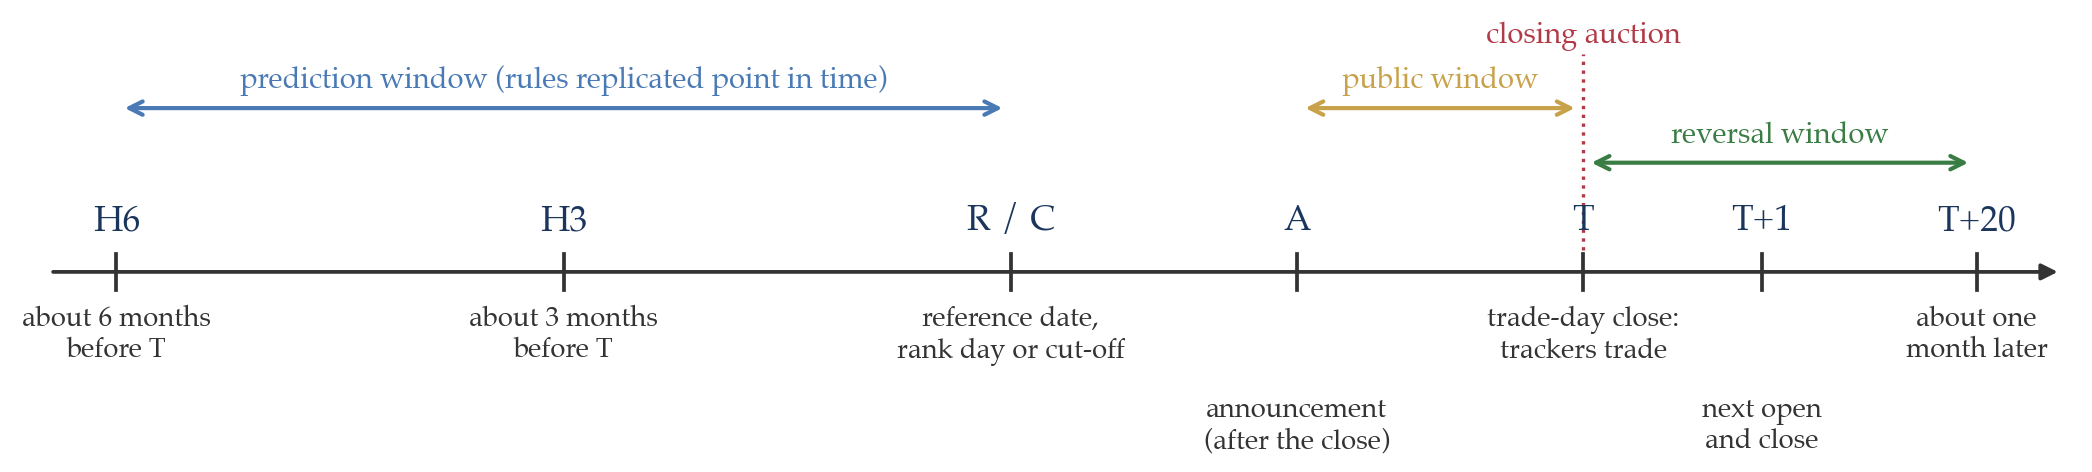
\includegraphics[width=0.9\textwidth]{figures/fig01_timeline.png}
\caption{Event timeline for one review (not to scale). Portfolios are formed at H6, H3 or the ranking date (R or C) and held to the trade-day close T; post-event legs run from T to the next open, the next close and T+20.}
\label{fig:timeline}
\qsource{provider calendars; author's design.}
\end{figure*}

\subsection{Point-in-time prediction}

At each horizon we apply the provider's current rules to every eligible stock using only data dated on or before that day: prices, volume, shares, float estimates, membership as known on the day (including changes already announced) and review results already published. For the Russell, companies are ranked by total market capitalisation summed across share classes, with the $\pm$2.5 percentile band at rank 1,000 and price, size and float screens; companies the rebuild ranked 1,001--2,700 at the previous rank day but which Russell still left out are treated as ineligible. For the S\&P/TSX the size, turnover, price and seasoning tests of Table~\ref{tab:rules} are applied with the rule parameters of each era. For the STOXX 600 the 550/750 buffer is applied to free-float capitalisation in euros. For the DAX family the Fast Exit, Fast Entry and regular rules are applied with three eras of member counts.

Free float comes from Datastream where strategic holdings are reported, otherwise from Worldscope closely held shares, otherwise 100\%. At H6 the S\&P/TSX and STOXX screens face a timing problem: the next review, $q{-}1$, falls between H6 and the target review $q$. A name is then predicted for $q$ if, under a driftless random walk for its relative size, the probability that it fails at $q{-}1$ and passes at $q$ is at least 10\%.

Two choices were made after seeing errors, and both are disclosed. For the S\&P/TSX, the main model adds a filter for pending takeover targets and a ``committee memory'' that drops names the screen passed at one of the last two announced reviews but which were not added (and members the screen failed but which were kept). For the STOXX 600, four eligibility proxies were added after the first run. Results without these choices are reported alongside.

\subsection{Returns, controls and inference}

The \emph{capturable} portfolio holds every predicted name, false positives included, from its formation close. The \emph{hindsight} portfolio holds the actual changes from the same date; it cannot be traded and is shown to measure selection. Abnormal returns are the stock's return minus the equal-weighted return of matched controls that were neither predicted nor changed at that review. Controls are matched on size decile and prior momentum: 10 size deciles $\times$ 5 prior-126-day return quintiles for the Russell, size decile $\times$ 6-month momentum tercile for the S\&P/TSX and the DAX family, and country $\times$ size $\times$ momentum for the STOXX 600. Russell returns are buy-and-hold abnormal returns (BHAR) on CRSP total returns, delisting-aware. The other studies sum daily abnormal returns into a cumulative abnormal return (CAR), with daily returns clipped to $[-50\%, +100\%]$. The two conventions are not strictly comparable in magnitude.

Standard errors are clustered by year for the Russell (one reconstitution a year) and by review elsewhere. Many windows, sides and splits are tested, so we treat $|t| < 2.5$ as suggestive. Every study reports medians and trimmed means next to the mean, and an early (2006/2008--2015) against a late (2016--2026) split.

\subsection{The close}

For the close we use the actual changes. Each leg is a matched-control abnormal return signed so that \emph{positive means the price moved in the direction of index demand}: up for index buying, down for index selling. A positive trade-day number is a dislocation that index funds pay; a negative number after T is a reversal that a liquidity provider on the other side earns. The legs are T$-$1 close to T close, T close to T+1 open, T+1 open to close, and sums of daily abnormal returns to T+5 and T+20. In the DAX family the side is the sign of net visible passive demand, because a promotion from MDAX to DAX is a net sale (DAX trackers are a smaller share of float than MDAX trackers). Opens come from CRSP, Compustat and the Datastream primary quote.

\subsection{Measuring demand}

Per-stock demand is measured from fully replicating ETF holdings just before and after each effective date. The fund's trade in stock $i$ is $h_{a,i}/c' - h_{b,i}$, where $h_b$ and $h_a$ are holdings before and after on one split basis and $c'$ removes the fund's own creations and redemptions at fixed prices. This captures additions, deletions, share and float updates and capping in one measure, and it is scaled up by the visible assets that track the same index. The multiplier $R$ is the slope of excess trade-day volume on visible holdings demand, with event-date fixed effects. Holdings reproduce the known changes: for S\&P/TSX daily pairs they find 180 of 181 review additions and 144 of 144 deletions.

\subsection{Capacity}

Capacity is computed at 10\% participation: each predicted name can absorb 10\% of its median daily value traded over the 63 sessions before formation, for every session from formation to T (for the Russell deletion short, ten sessions at 10\%). The sum over a review's predicted names is the deployable amount; multiplying it by the measured mean return gives a gross figure before spreads, impact, taxes and borrow. We also report the result when each name's return is weighted by its deployable amount, which shows whether the liquid names earn the return.

%═══════════════════════════════════════════════════════
\section{Results}
\label{sec:results}

\subsection{How large the forced flow is}

Table~\ref{tab:demand} summarises the size of index demand. Visible passive shares are small, from 0.27\% of float for the STOXX 600 to 4.39\% for MSCI Europe Standard, but excess trade-day volume is several times the visible demand. In the S\&P/TSX the multiplier $R$ fell from 15.8 in 2012--2015 to 6.2 in 2023--2026 (Figure~\ref{fig:passive}a) while the visible ETF share rose from 0.15\% to 1.00\% of float, so the implied true share rose only from about 2.4\% to 6.2\%. MSCI's visible share is much larger than an ETF-only proxy suggests, because World, ACWI and EAFE funds hold the same names (Figure~\ref{fig:passive}b): only about a quarter of the Canadian figure sits in MSCI Canada country funds.

\begin{table}[t]
\centering
\caption{Passive demand by index. Visible $\pi$ is \% of float held by observable trackers; $R$ is true over visible demand from excess trade-day volume; true $\pi = R \times$ visible $\pi$ (an upper bound on index-fund ownership).}
\label{tab:demand}
\footnotesize
\qstripes
\begin{tabularx}{\columnwidth}{@{}Xrrr@{}}
\toprule
\qhead{Index (latest window)} & \qhead{Vis.\ $\pi$} & \qhead{$R$} & \qhead{True $\pi$} \\
\midrule
S\&P/TSX Composite (2023--26) & 1.00\% & 6.2 & 6.2\% \\
Russell 2000 & -- & 5.1 & 15.7\% \\
S\&P 500 (2023--25) & -- & 6.4 & 26\% \\
STOXX Europe 600 & 0.27\% & 3.9 & 1.1\% \\
MSCI Canada Standard (Jul 2026) & 1.58\% & 7.15 & 11.3\% \\
MSCI Europe Standard (Jul 2026) & 4.39\% & 2.45 & 10.7\% \\
\bottomrule
\end{tabularx}
\vspace{2pt}

\parbox{\columnwidth}{\footnotesize STOXX 600 and MSCI Europe $R$ use primary-venue volume only and are lower bounds on the volume-implied share; the STOXX 600 $R$ ranges 3.9--5.4 across the estimates reported. The Russell 2000 and S\&P 500 visible shares are time-varying and are not shown.}
\qsource{iShares holdings files; Thomson mutual-fund holdings, Datastream and Compustat volume via WRDS; author's calculations.}
\end{table}

\begin{figure*}[t]
\centering
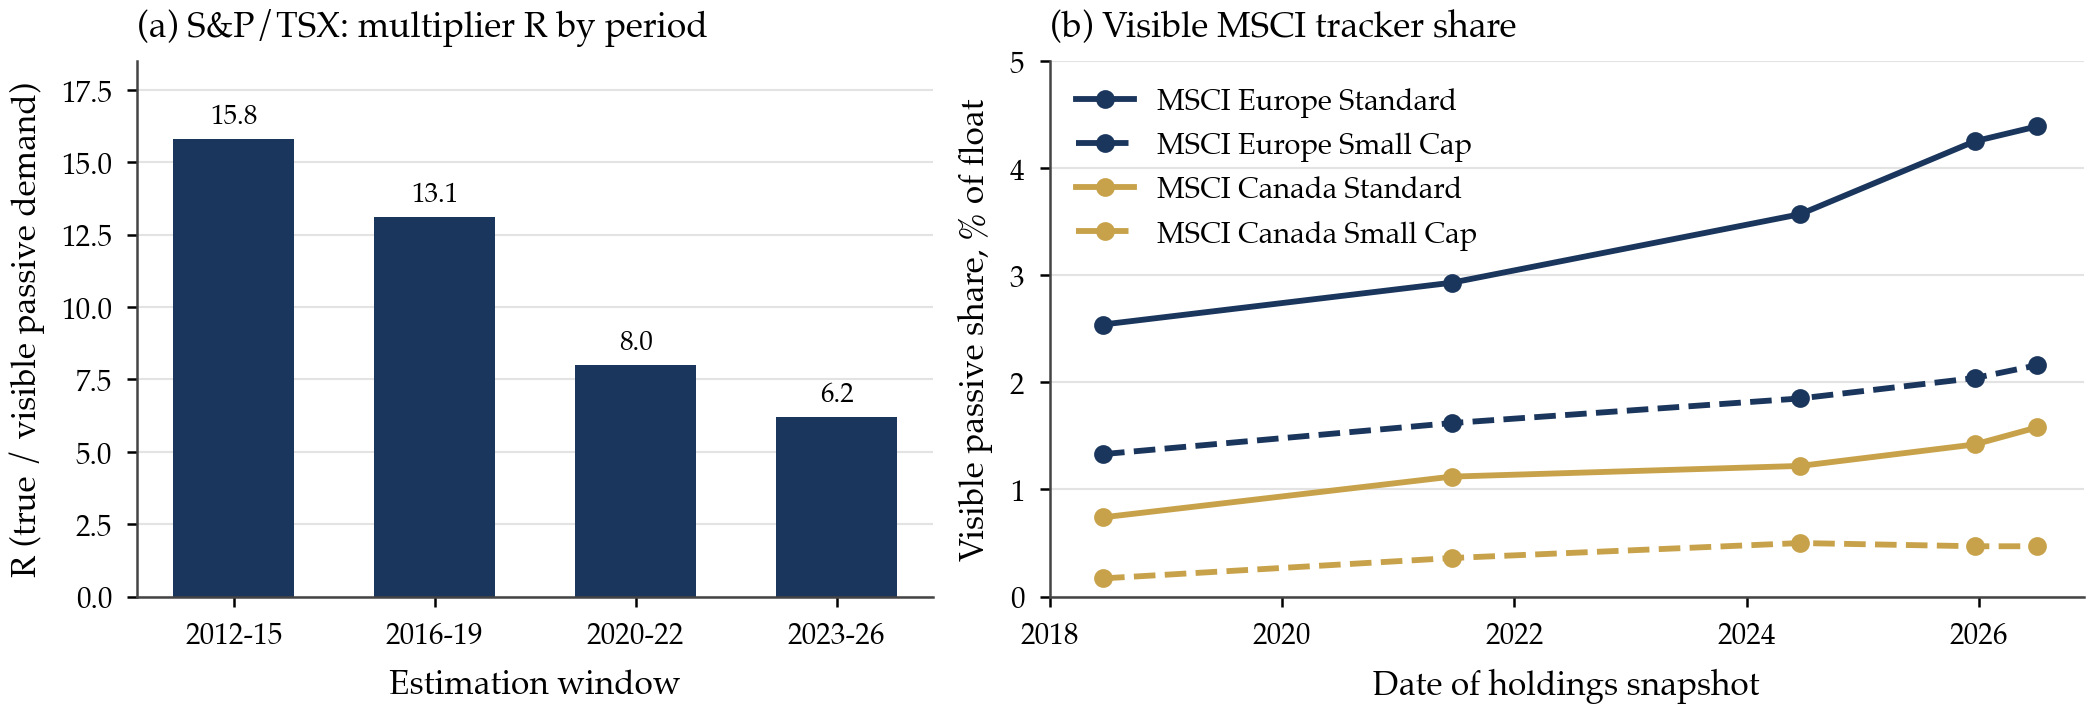
\includegraphics[width=0.92\textwidth]{figures/fig02_passive.png}
\caption{(a) Ratio of true to visible passive demand for S\&P/TSX Composite events, by estimation window (2012--2026), from excess trade-day volume with event-date fixed effects. (b) Visible passive share of four MSCI segments, June 2018 to July 2026, from every visible tracker that holds the segment's names, \% of the segment's float.}
\label{fig:passive}
\qsource{iShares holdings files; Thomson mutual-fund holdings and Datastream volume via WRDS; author's calculations.}
\end{figure*}

The trade-day volume confirms the flow. In 2016--2025 actual Russell additions traded a median 15.8$\times$ their normal volume on reconstitution day and deletions 13.8$\times$, against 2.3$\times$ for controls. S\&P/TSX additions traded 7.1$\times$ on consolidated Canadian volume (11.1$\times$ on TSX-only volume) and the TSX's share of consolidated volume rose from 59\% to 89\% on the day, which is the closing auction. In Canada the median excess trade-day volume of an MSCI Standard/Small Cap migration is 6.9\% of index float, or 9.9$\times$ the 60-day average.

Weight changes in existing members are a second source of flow. In Canada they came to a median C\$1.36bn across 71 names per review since 2016, 3.1 times the notional of additions and deletions, but only 0.27$\times$ average daily volume for the median name. In the Russell they are 0.36 times the reconstitution flow, though 441 names a year carry more than one day's volume.

\subsection{How well the changes can be predicted}

Figure~\ref{fig:acc} shows precision (the share of predicted changes that happened) and recall (the share of actual changes predicted). Accuracy improves sharply as the ranking date approaches. Six months out, the problem for the S\&P/TSX is \emph{which review}: of the names predicted at H6 for review $q$, only 8\% changed at $q$, a further 7\% at $q{-}1$, 8\% at $q{+}1$ and 11\% at $q{+}2$ to $q{+}4$, while 65\% never changed. For the STOXX 600 the binding problem at the cut-off is false positives: the rules predict 24 additions per review against 8.7 actual, and names whose float defaults to 100\% have 5\% add precision. Even at the Russell rank day add precision is 65\%, because Russell's country, float, voting-rights and share-class judgements are not observable in our data.

\begin{figure*}[t]
\centering
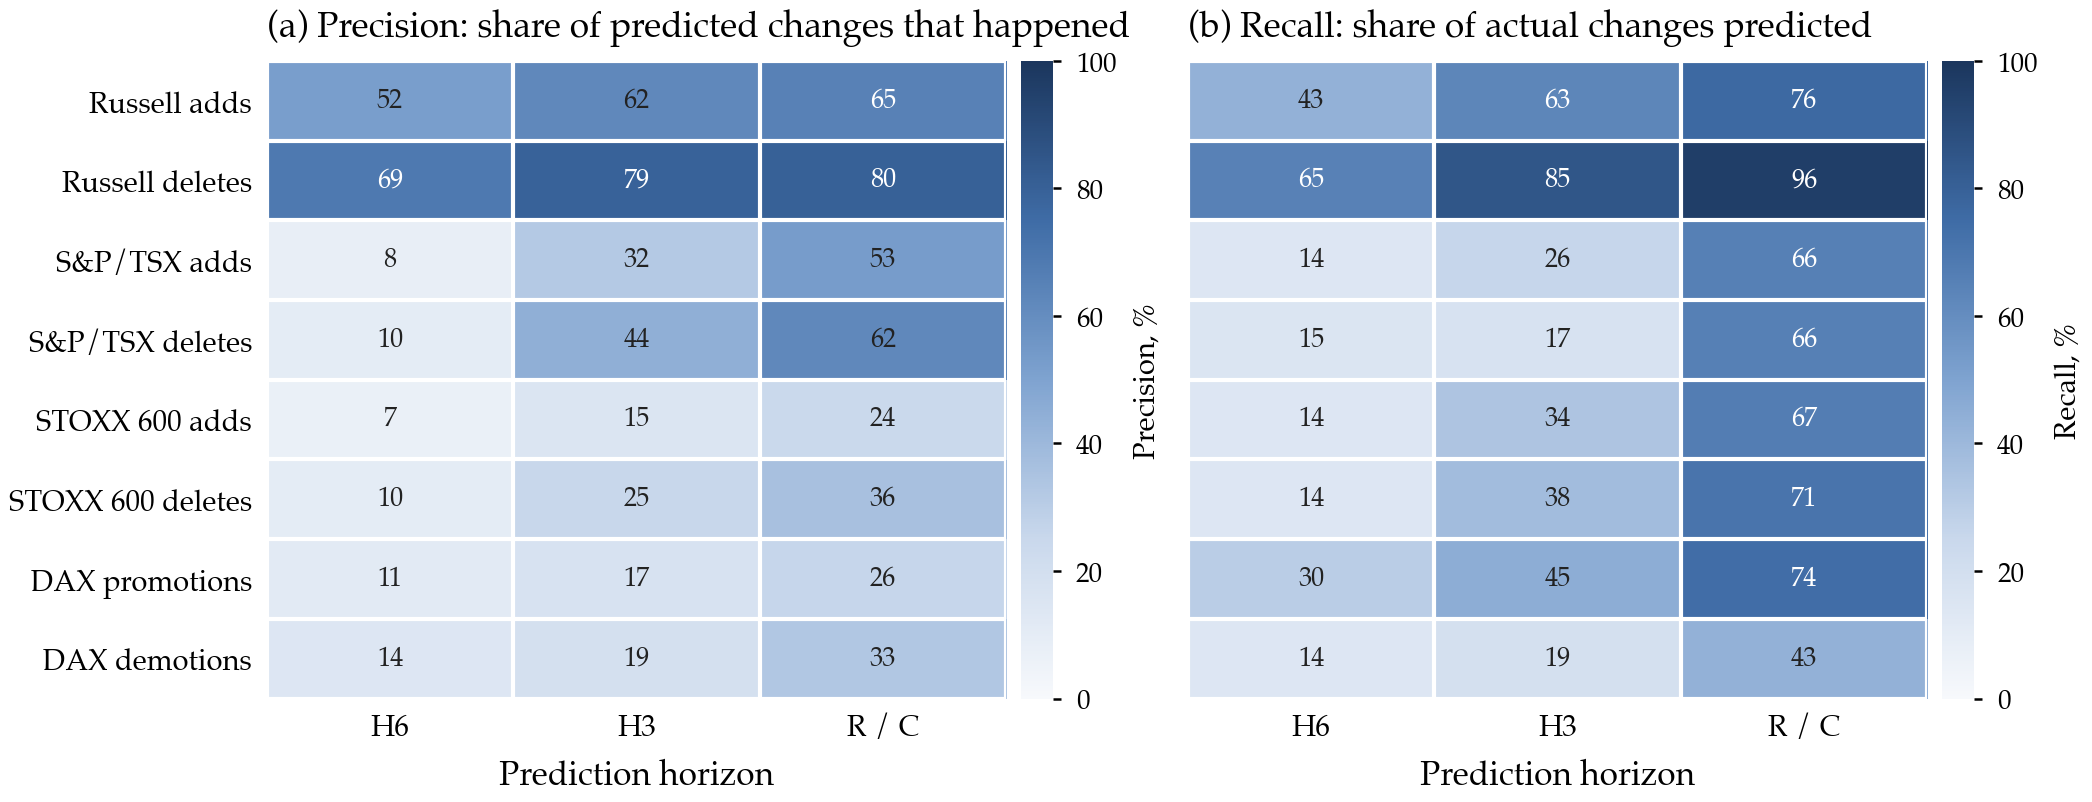
\includegraphics[width=0.92\textwidth]{figures/fig03_accuracy.png}
\caption{Prediction accuracy by family, side and horizon: (a) precision, the share of predicted changes that happened; (b) recall, the share of actual changes predicted. Russell 2016--2025 (new R2000 additions; R2000 deletions); S\&P/TSX main model 2006--2026; STOXX 600 and DAX family rules model 2008--2026. A naive size rule reaches 6--10\% for S\&P/TSX additions and 2--4\% for STOXX 600 additions.}
\label{fig:acc}
\qsource{CRSP, Compustat and Datastream via WRDS; author's calculations.}
\end{figure*}

\subsection{Selection is not a capturable premium}

Names that were actually added rose strongly before the event, and names that were deleted fell (Figure~\ref{fig:select}). From six months out, actual S\&P/TSX additions beat controls by 36.4\% and actual deletions lagged by 47.3\%. These moves are the reason the names changed: the size test selects on exactly these returns. A trader at H6 or H3 cannot tell which near-threshold names will keep moving. In the STOXX 600 the 89 predicted additions that were then added earned +23.4\% from six months out; the 1,265 that were not earned $-$0.3\%. At 7--17\% precision six and three months out, the true positives are too few to lift the portfolio.

\begin{figure*}[t]
\centering
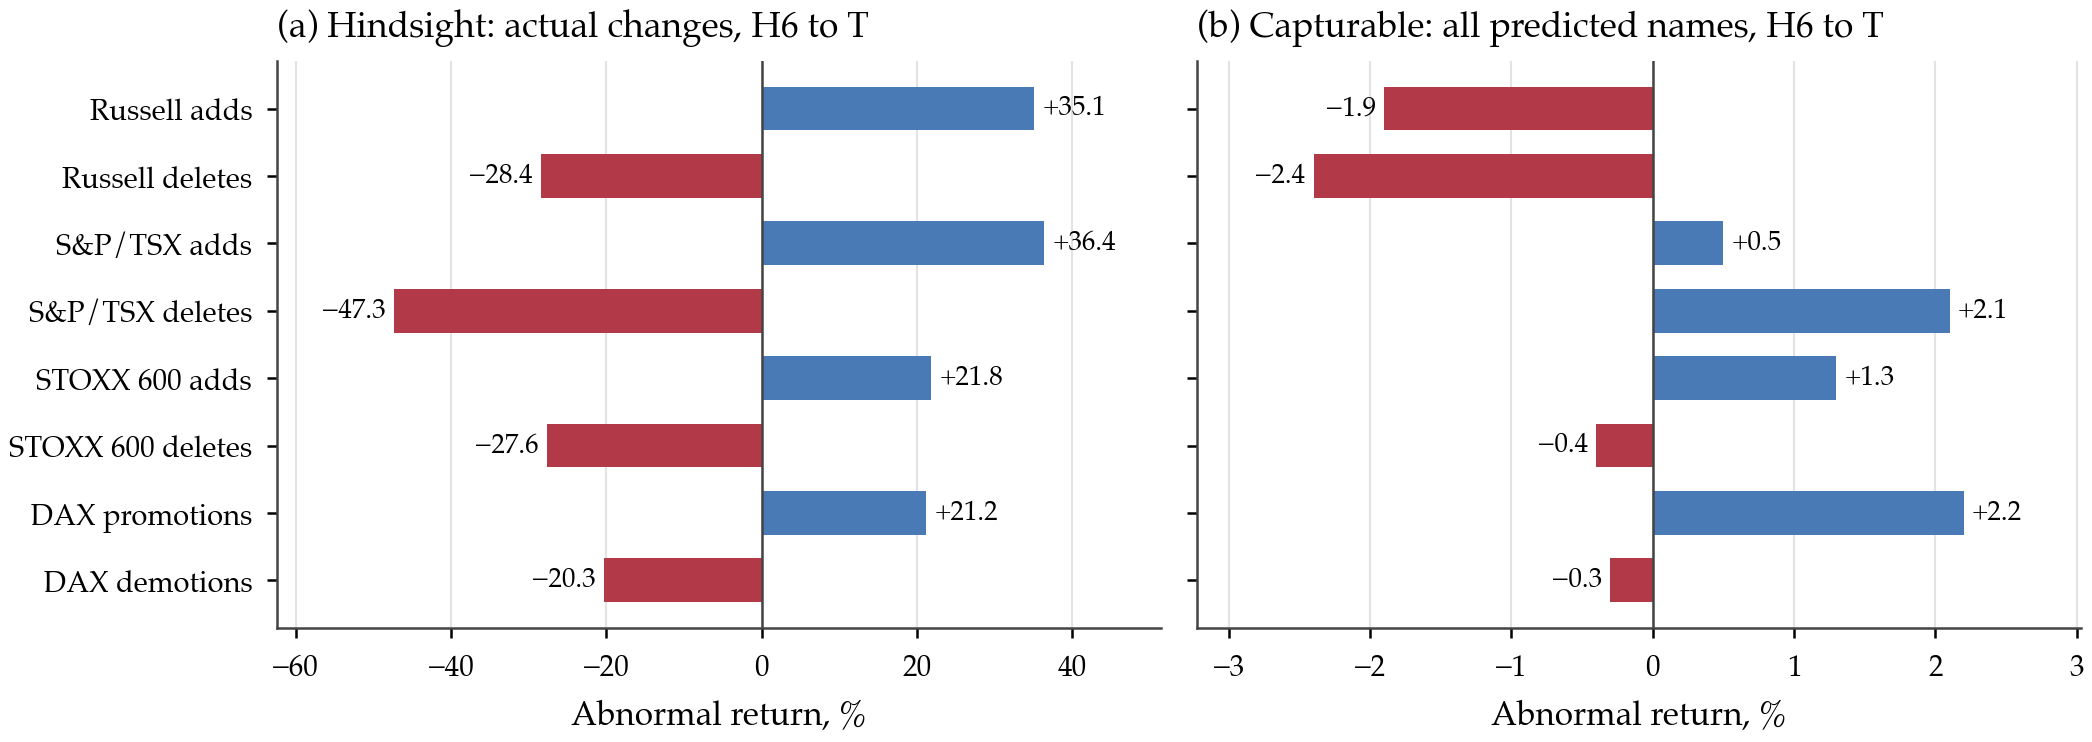
\includegraphics[width=0.8\textwidth]{figures/fig04_selection.png}
\caption{Hindsight against capturable returns from six months out (H6) to the trade close. (a) The actual changes; (b) every predicted name, false positives included. Russell 2016--2025 buy-and-hold abnormal returns; other families full-sample matched-control CARs (S\&P/TSX 2006--2026, STOXX 600 2008--2026, DAX family 2008--2025).}
\label{fig:select}
\qsource{CRSP, Compustat and Datastream via WRDS; author's calculations.}
\end{figure*}

\subsection{Russell June reconstitution}

Table~\ref{tab:russell} and Figures~\ref{fig:rus16}--\ref{fig:rusheat} show the capturable Russell portfolios. In 2016--2025, predicted additions gained +2.5\% from end-December to end-March and then gave it back: from rank day to the reconstitution close they lost 4.0\% against controls ($t = -2.0$; $-$5.5\% trimmed). Over the whole hold from end-December they returned $-$1.9\%. This is not a prediction failure: with hindsight, actual additions held from rank day also lost 2.3\%. Shorting predicted deletions from end-December earned 2.4\% on the mean, but the median deletion fell 12.1\% against controls; the mean is pulled down by a fat right tail, which is what a short would have paid. From rank day the short earned nothing. After the close, rank-day-predicted deletions rebounded +3.2\% over 20 trading days ($t = 2.1$) and +5.2\% over 60.

\begin{table}[t]
\centering
\caption{Russell capturable portfolios, abnormal BHAR \% (t clustered by year). For deletes a negative return is a profit for the short.}
\label{tab:russell}
\footnotesize
\qstripes
\begin{tabularx}{\columnwidth}{@{}Xrr@{}}
\toprule
\qhead{Portfolio, window} & \qhead{2016--25} & \qhead{2008--15} \\
\midrule
Adds, end-Dec $\to$ end-Mar & +2.5 (1.3) & +3.2 (1.8) \\
Adds, end-Dec $\to$ recon close & \mn1.9 (\mn0.5) & +6.7 (2.3) \\
Adds, rank day $\to$ recon close & \mn4.0 (\mn2.0) & +1.0 (0.6) \\
Deletes, end-Dec $\to$ recon close & \mn2.4 (\mn0.7) & +1.3 (0.1) \\
\quad median & \mn12.1 & \mn13.3 \\
Deletes, rank day $\to$ recon close & +0.6 (0.25) & \mn5.0 (\mn3.2) \\
Deletes (rank day), close $\to$ +20 days & +3.2 (2.1) & +1.6 (0.6) \\
Adds (rank day), close $\to$ +60 days & \mn1.0 (\mn0.9) & \mn7.8 (\mn3.1) \\
\bottomrule
\end{tabularx}
\qsource{CRSP and Datastream Russell constituent lists via WRDS; author's calculations.}
\end{table}

\begin{figure*}[t]
\centering
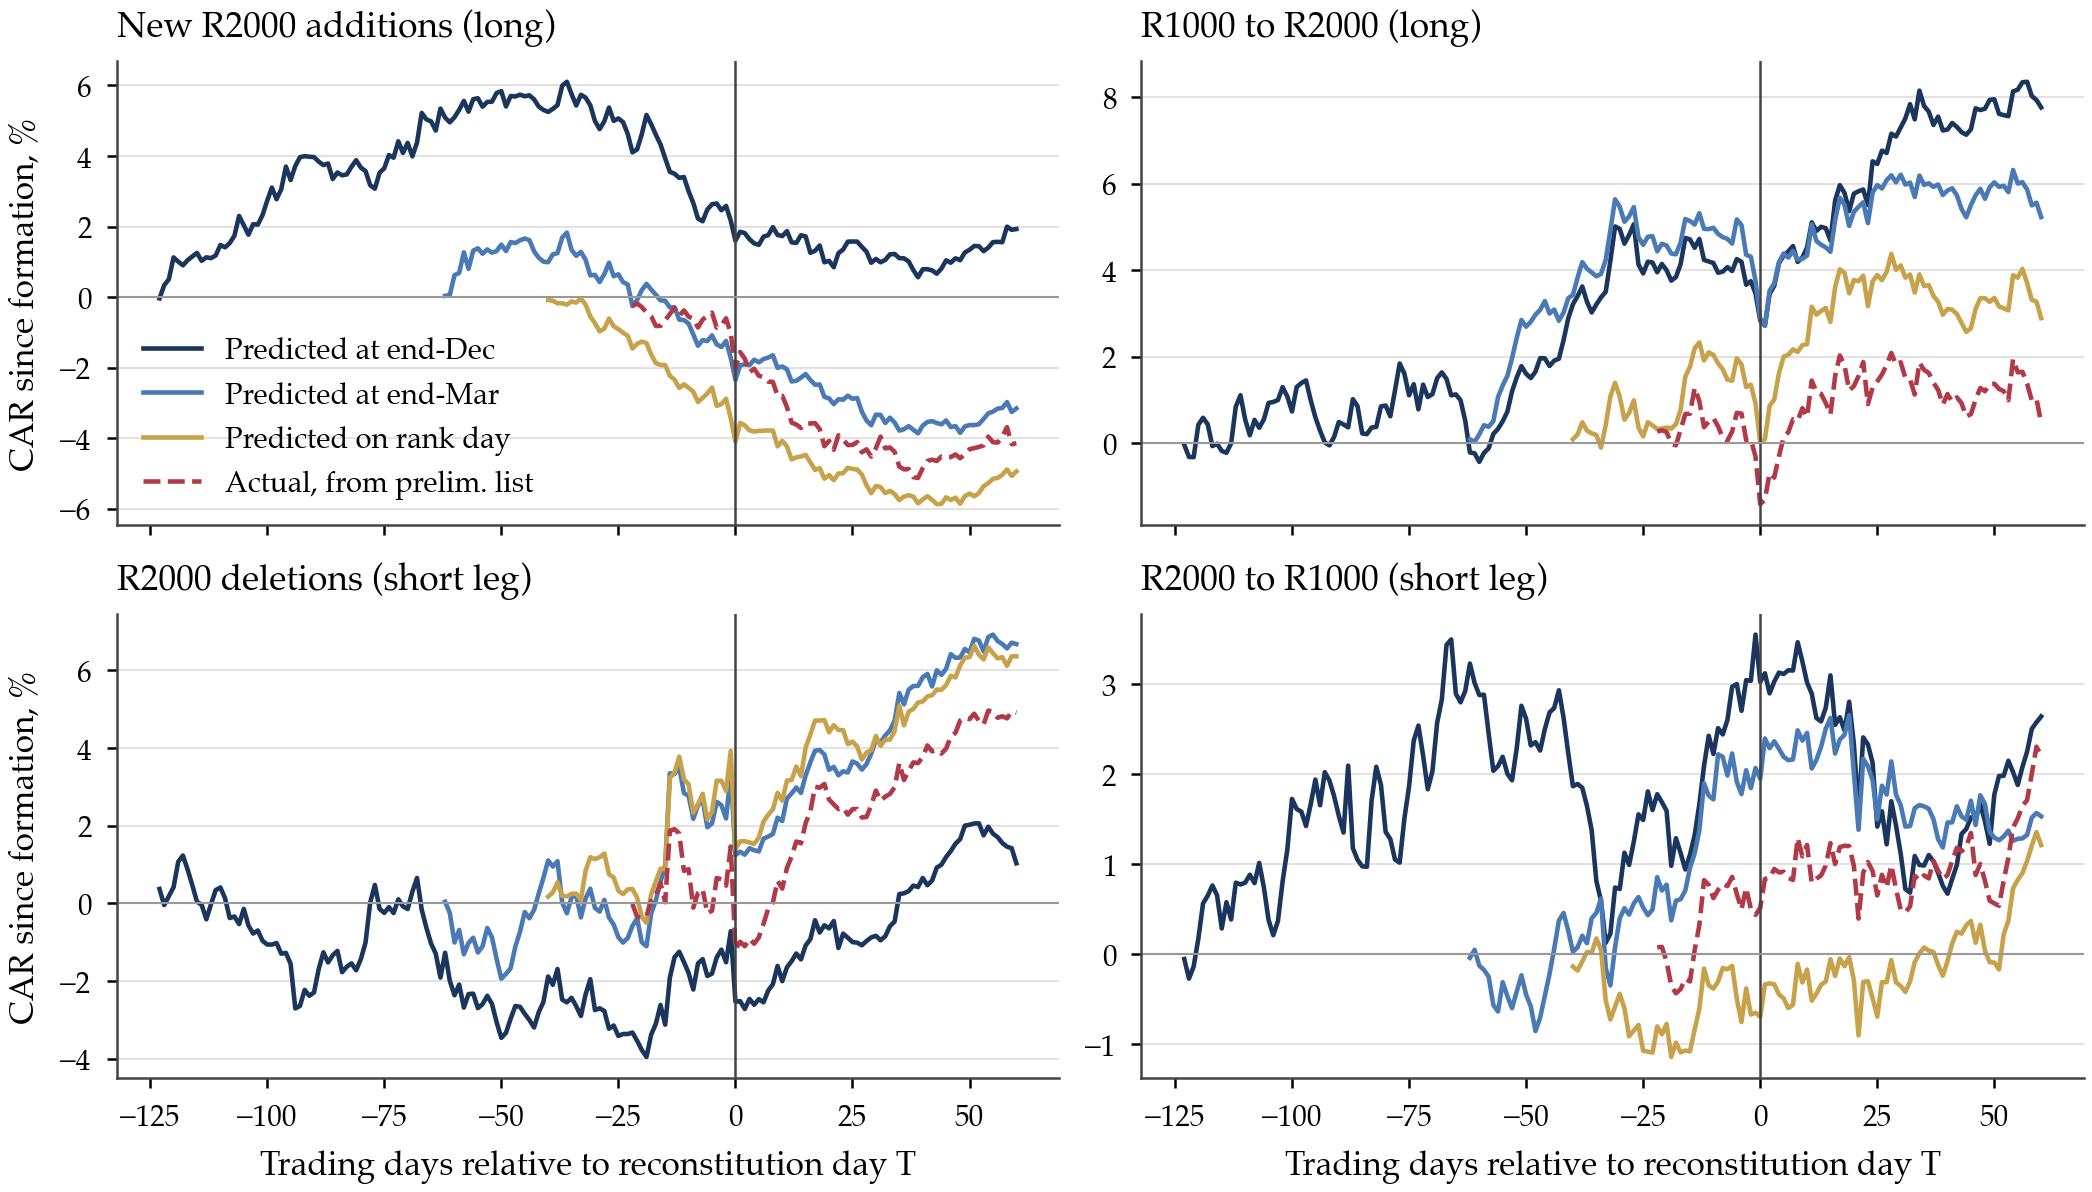
\includegraphics[width=0.8\textwidth]{figures/fig_russell_paths_2016_2025.png}
\caption{Russell, 2016--2025: cumulative abnormal return of each capturable portfolio from its own formation close (end-December, end-March, rank day), and of the actual changes from the preliminary-list close, against trading days relative to the reconstitution day T. Each year's daily mean abnormal return is cumulated from its formation day and the paths are averaged across years, which for these small caps runs above the buy-and-hold figures in Table~\ref{tab:russell}.}
\label{fig:rus16}
\qsource{CRSP and Datastream Russell constituent lists via WRDS; author's calculations.}
\end{figure*}

\begin{figure*}[t]
\centering
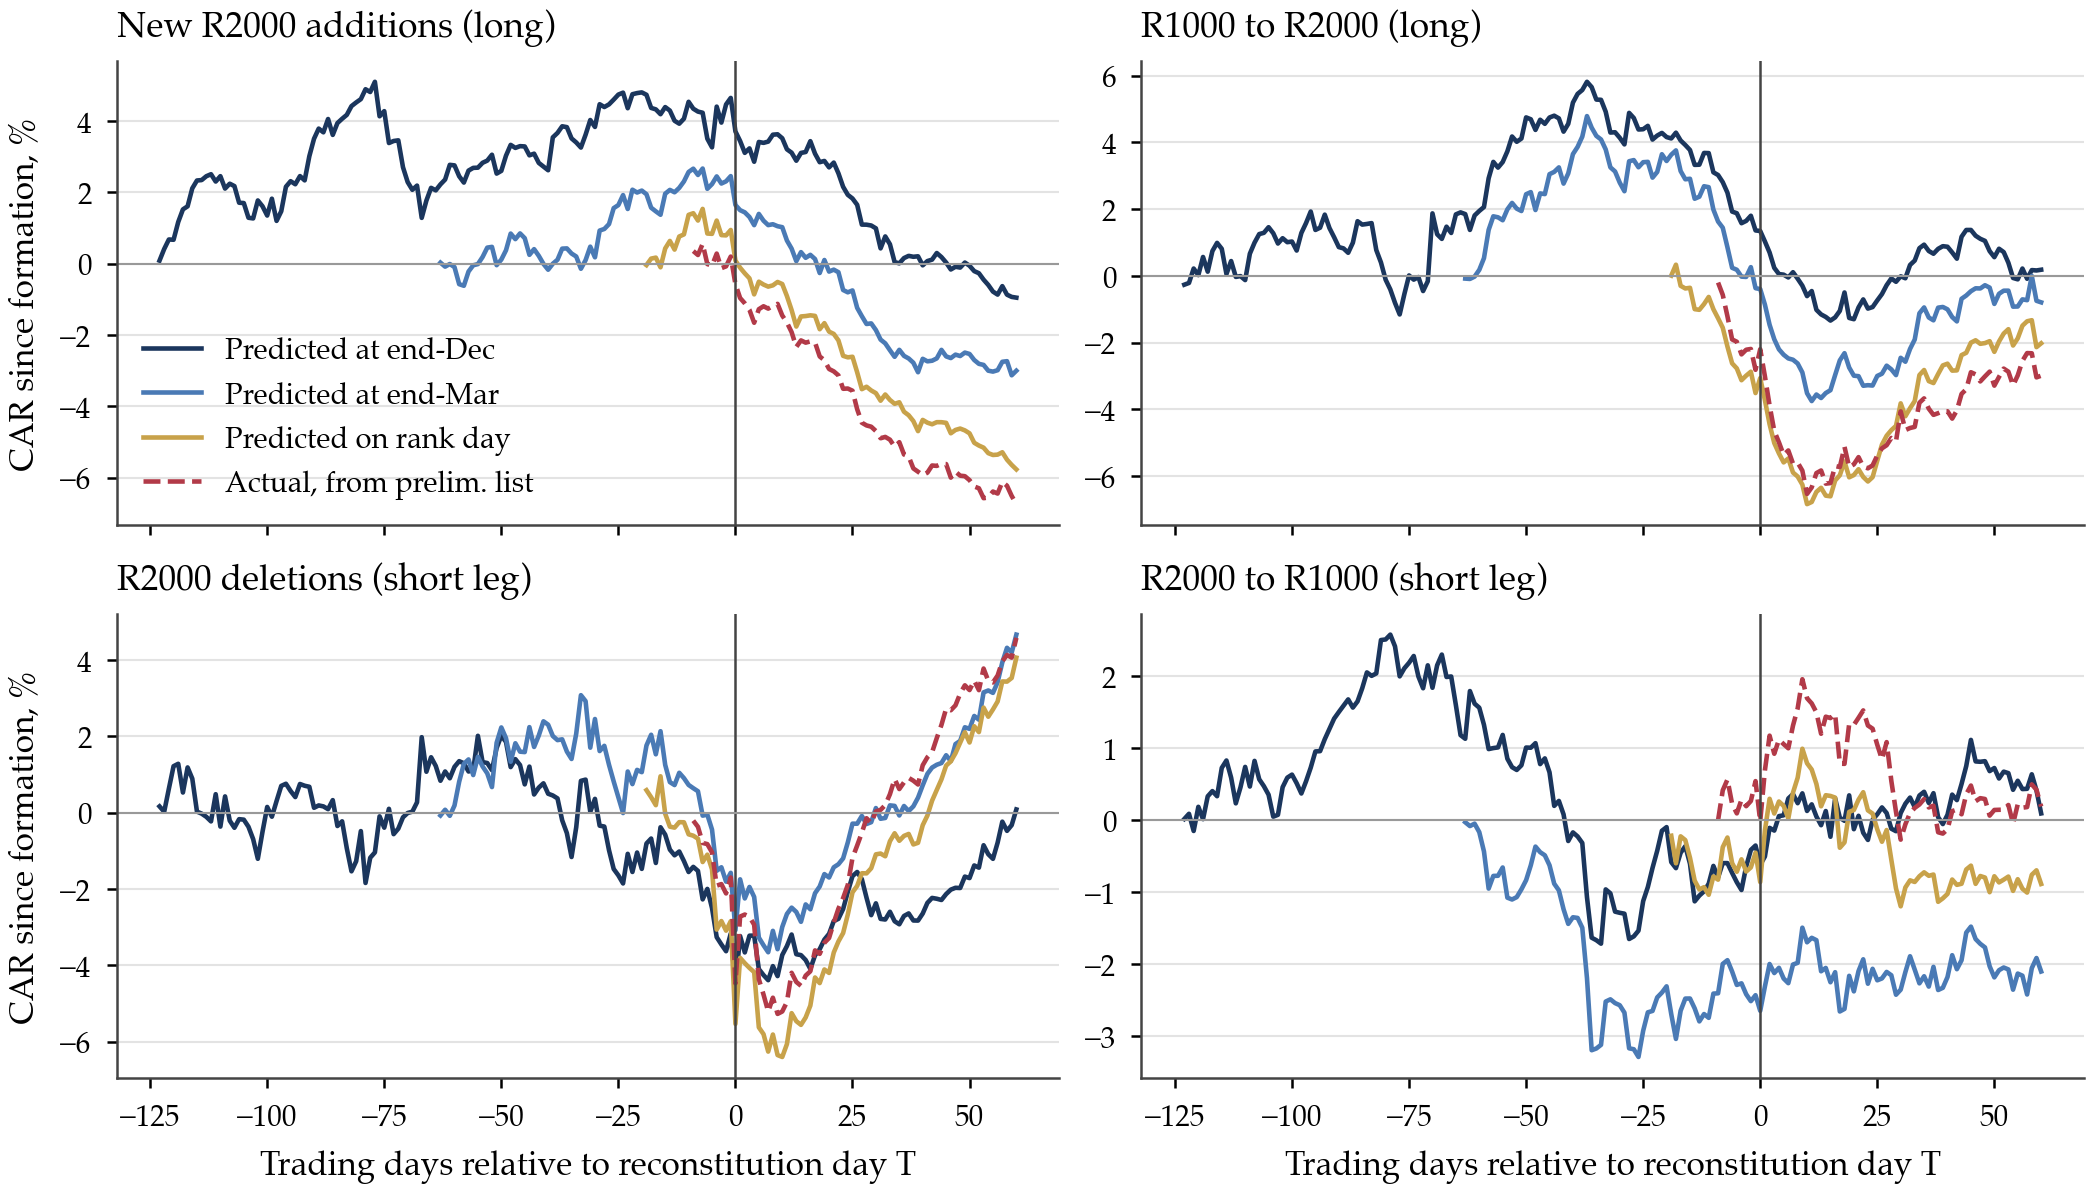
\includegraphics[width=0.8\textwidth]{figures/fig_russell_paths_2008_2015.png}
\caption{Russell, 2008--2015: the same capturable portfolios as Figure~\ref{fig:rus16}. Before 2016 predicted additions held their gains into the reconstitution close and predicted deletions fell into it.}
\label{fig:rus08}
\qsource{CRSP and Datastream Russell constituent lists via WRDS; author's calculations.}
\end{figure*}

\begin{figure*}[t]
\centering
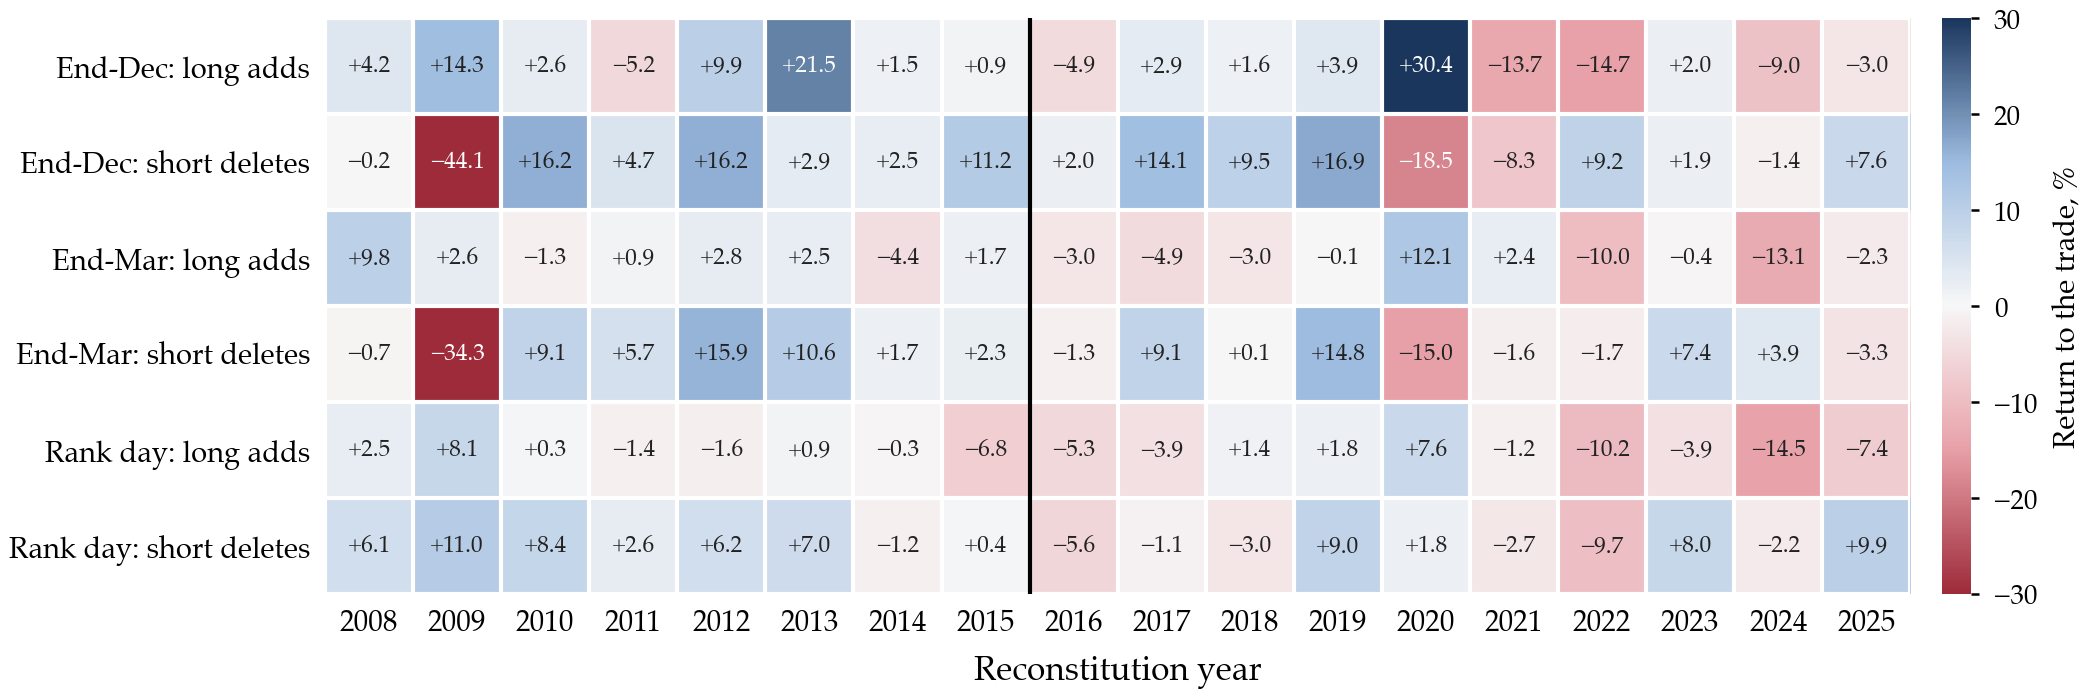
\includegraphics[width=0.92\textwidth]{figures/fig_russell_heat.png}
\caption{Russell capturable portfolios by reconstitution year, 2008--2025: mean buy-and-hold abnormal return from each formation date to the reconstitution close, signed as the return to the trade (long predicted additions, short predicted deletions), \%. The vertical line separates the early and late samples; colours are capped at $\pm$30\%.}
\label{fig:rusheat}
\qsource{CRSP and Datastream Russell constituent lists via WRDS; author's calculations.}
\end{figure*}

The same trade worked in 2008--2015. Predicted additions held from end-December earned +6.7\% ($t = 2.3$, 7 of 8 years positive) and shorting predicted deletions from rank day earned 5.0\% ($t = 3.2$). Figure~\ref{fig:rusheat} shows the year-by-year pattern behind these averages. The equal-weighted long-short spread from end-December averaged +6.5\% per reconstitution in 2008--2015 and +2.7\% in 2016--2025 ($t = 0.8$, 7 of 10 years positive); from rank day it was +3.9\% and $-$2.5\%.

\subsection{S\&P/TSX Composite}

Over the full sample, predicting the Composite months ahead earned roughly nothing: predicted additions beat controls by +0.5\% from H6 and +2.0\% from H3, and predicted deletions \emph{rose}, so the short lost. The split at 2016 changes the reading (Table~\ref{tab:tsx}). Before 2016 the classic price-pressure pattern was there: from the reference date, predicted additions earned +1.5\% to the trade close and predicted deletions lost 4.7\%, and both then reversed. Since 2016 those effects are gone or reversed, and actual deletions now rebound +5.7\% between the reference date and the announcement, which suggests early shorts covering before the event.

\begin{table}[t]
\centering
\caption{S\&P/TSX Composite capturable portfolios by period, matched-control CAR \% (t clustered by review).}
\label{tab:tsx}
\footnotesize
\qstripes
\begin{tabularx}{\columnwidth}{@{}Xrr@{}}
\toprule
\qhead{Portfolio, window} & \qhead{2006--15} & \qhead{2016--26} \\
\midrule
Pred.\ adds, H6 $\to$ T & +1.8 (1.0) & \mn1.3 (\mn0.5) \\
Pred.\ adds, H3 $\to$ T (main model) & \mn0.4 (\mn0.2) & +6.8 (3.3) \\
Pred.\ adds, H3 $\to$ T (rules only) & \mn0.6 & +3.4 (2.4) \\
Pred.\ adds, R $\to$ T & +1.5 (2.0) & \mn0.8 (\mn0.6) \\
Pred.\ deletes, R $\to$ T & \mn4.7 (\mn3.1) & +2.6 (1.2) \\
Actual deletes, R $\to$ A & \mn2.8 (\mn1.6) & +5.7 (2.2) \\
Actual deletes, T $\to$ T+20 & +9.4 (2.4) & \mn1.2 (\mn0.6) \\
Actual adds, T $\to$ T+20 & \mn3.1 (\mn3.6) & +1.4 (0.9) \\
\bottomrule
\end{tabularx}
\qsource{Compustat index constituents and prices, Datastream volume and free float via WRDS; author's calculations.}
\end{table}

\begin{figure*}[t]
\centering
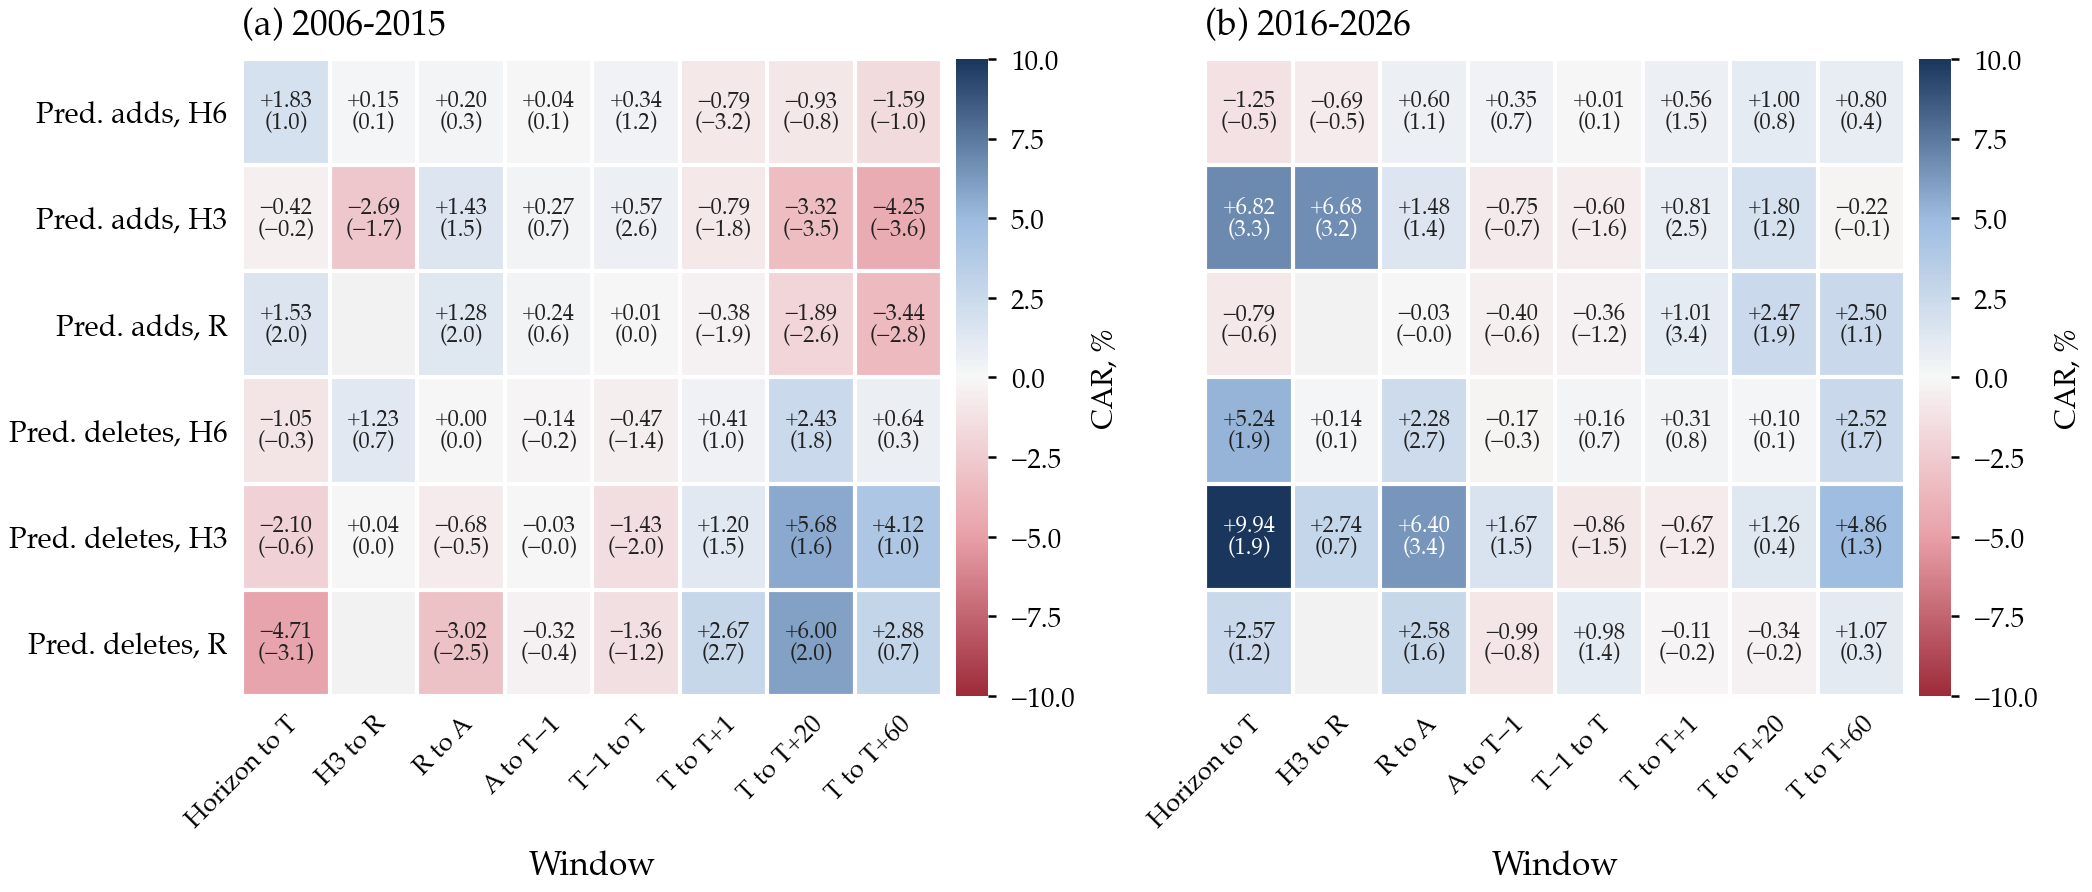
\includegraphics[width=0.92\textwidth]{figures/fig_tsx_segments.png}
\caption{S\&P/TSX Composite: where the capturable return is earned. Matched-control CAR, \% (t-statistic clustered by review), of predicted additions and deletions formed at H6, H3 and the reference date R, from formation to T and by window: H3 to R, R to the announcement A, A to T$-$1, the trade day, and after T. (a) 2006--2015; (b) 2016--2026. For deletions a negative return is a profit for a short. Colours capped at $\pm$10\%.}
\label{fig:tsxseg}
\qsource{Compustat index constituents and prices, Datastream volume and free float via WRDS; author's calculations.}
\end{figure*}

The one surviving pocket is additions predicted three months out (Figure~\ref{fig:tsxseg}): +6.8\% in 2016--2026 under the main model ($t = 3.3$, $n = 102$ names over 36 reviews, median +5.3\%). It survives a 10\% trim (+6.3\%) and dropping 2025--26 (+5.7\%, $n = 88$), and 75\% of reviews were positive. Almost all of it (+6.7\%) is earned between H3 and the reference date, and none of it reverses within 60 sessions, which looks like a premium for positioning early rather than a close effect. Because the main model's filters were set after seeing errors, the plain rules screen is the more honest number: +3.4\% ($t = 2.4$, $n = 181$). Six-month prediction is not usable without a model of review timing.

\subsection{STOXX Europe 600 and the DAX family}

Predicting the STOXX 600 months ahead earns nothing reliable (Figure~\ref{fig:cross}). Predicted additions earned +1.3\% from six months out ($t = 1.4$, $n = 1{,}354$; median +2.0\%), $-$0.5\% from three months out and $-$0.6\% from the cut-off ($t = -2.8$). Predicted deletions show nothing at any horizon. After the cut-off, actual additions lost money into the close, almost all of it in the UK: UK additions fell 1.3\% on the trade day ($t = -4.1$) and UK deletions rose 1.0\% ($t = 2.9$). Shorting deletions predicted three months out paid only in markets without a share-purchase tax: $-$3.0\% ($t = -3.0$, $n = 561$), of which $-$4.4\% in 2008--2015 and $-$1.3\% ($t = -1.3$) in 2016--2026.

The DAX family pays a little from months out. Predicted promotions earned +2.2\% from six months out over the full sample ($t = 2.4$, $n = 939$) and +3.1\% in 2016--2026 ($t = 2.7$). The return sits in small names: in 2016--2026, predicted SDAX entries (median market capitalisation \texteuro0.86bn) earned +5.0\% from six months out ($t = 2.5$) and TecDAX entries +6.8\% ($t = 2.2$), while predicted promotions into the DAX itself earned $-$1.6\% (Figure~\ref{fig:dax}). Predicted demotions show no edge.

\begin{figure*}[t]
\centering
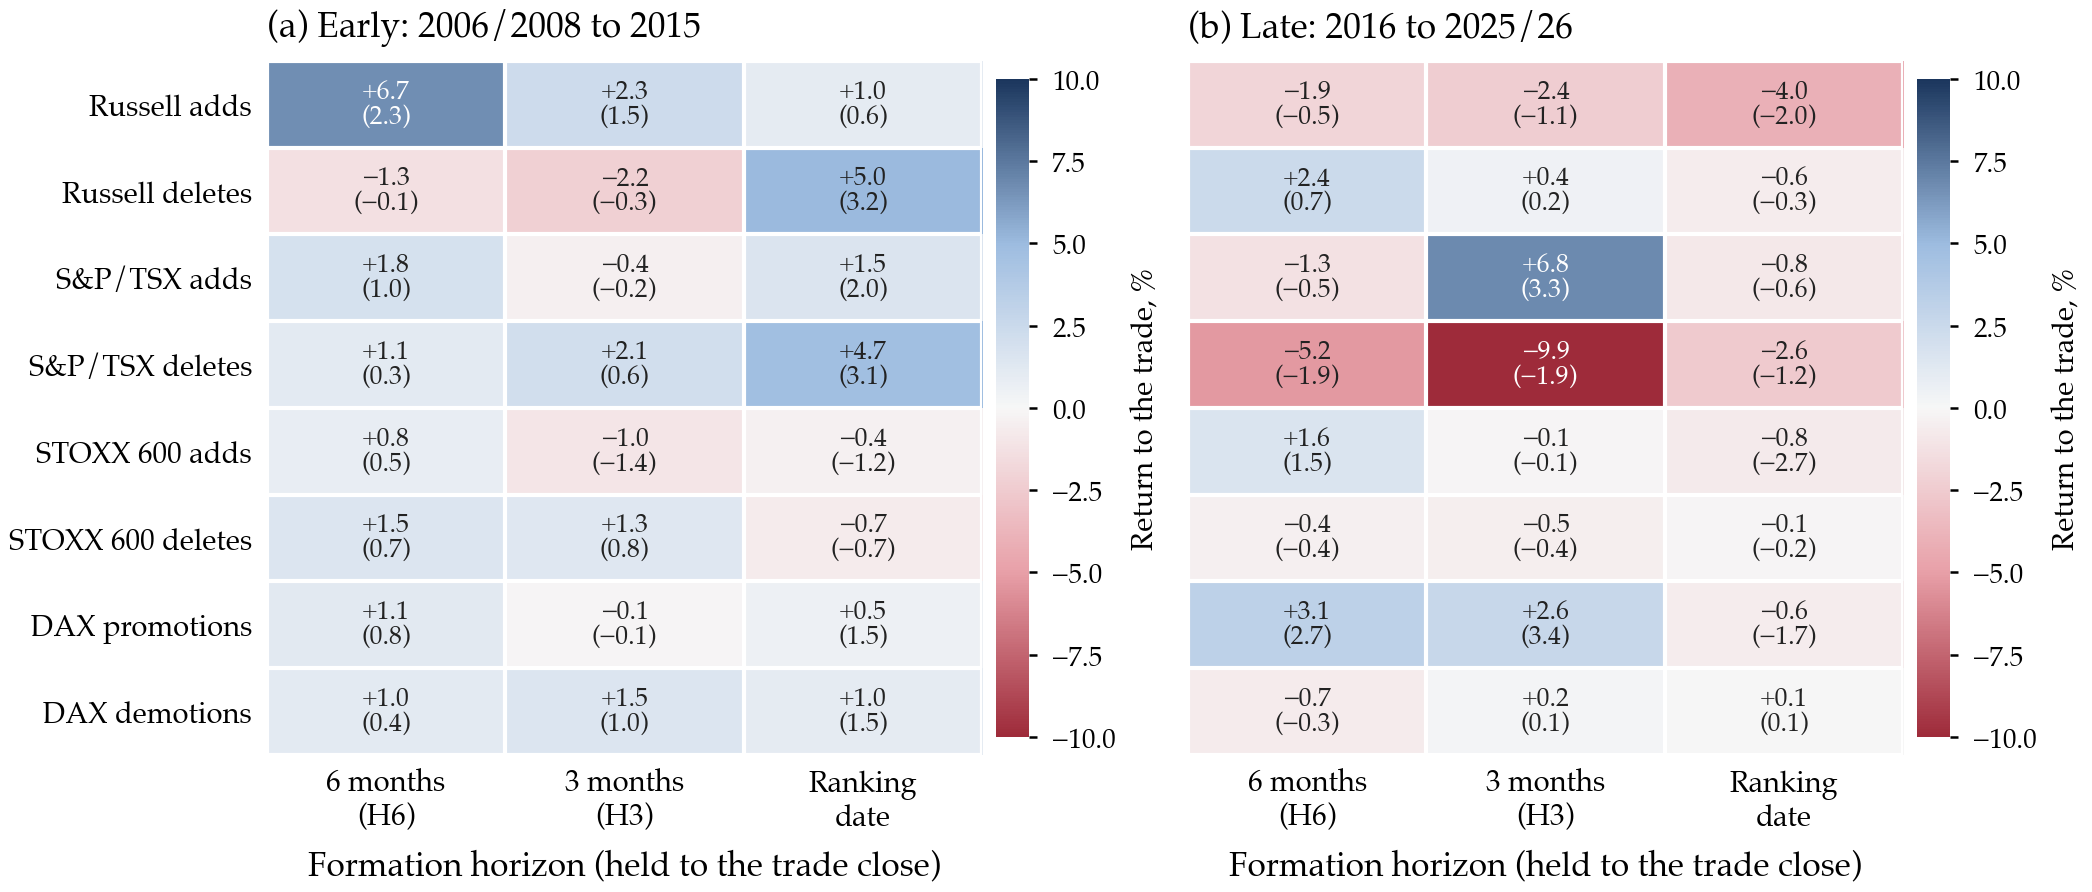
\includegraphics[width=0.92\textwidth]{figures/fig_cross_market.png}
\caption{Capturable return by family, side and formation horizon, held to the trade close, \% (t-statistic in brackets), signed as the return to the trade (long additions and promotions, short deletions and demotions). (a) 2006--2015 for the S\&P/TSX and 2008--2015 for the others; (b) 2016 to 2025 (Russell) or 2026. Russell figures are buy-and-hold abnormal returns; the others are matched-control CARs. S\&P/TSX uses the main model.}
\label{fig:cross}
\qsource{CRSP, Compustat and Datastream via WRDS; author's calculations.}
\end{figure*}

\begin{figure}[t]
\centering
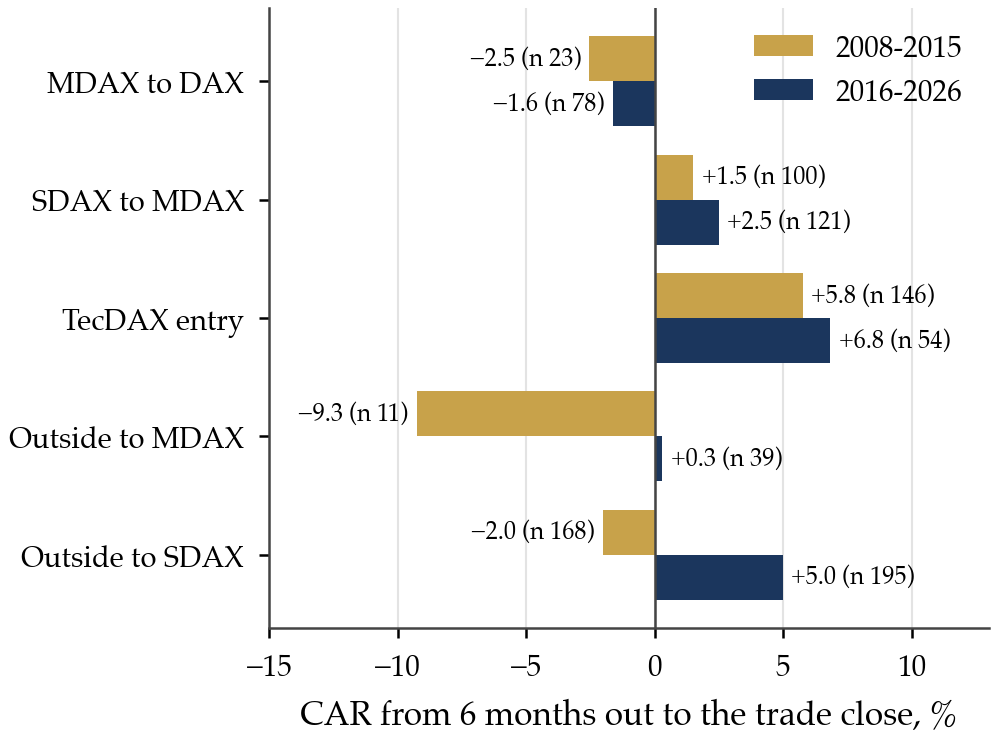
\includegraphics[width=\columnwidth]{figures/fig_dax_target.png}
\caption{DAX family: CAR of predicted promotions from six months out to the trade close by target index, 2008--2015 against 2016--2026, with the number of predicted names.}
\label{fig:dax}
\qsource{Compustat Global, Datastream constituent lists, volume and free float, and Worldscope via WRDS; author's calculations.}
\end{figure}

\subsection{Footprints of pre-positioning}

If traders position months ahead, their positions should be visible. We tracked the combined 13F long holdings of fourteen hedge-fund families, mostly multi-manager platforms and quantitative or market-making firms, identified by their 13F filer numbers. In Russell names predicted to join the R2000, their median combined holding rose from 0.55\% of shares in September to 0.75\% in December and 1.42\% at the March quarter-end (on the mean, 1.00 percentage point above matched controls), and fell back to 0.77\% just after the June reconstitution. In predicted deletions their holdings jumped from 0.45\% in March to 1.38\% at the June quarter-end, as they bought from index funds at the close. Short interest in predicted deletions rose from 2.26\% of shares at end-December to 4.02\% in mid-June and fell to 1.52\% by end-July. Turnover in predicted additions ran 23--54\% above baseline from December to May. Figure~\ref{fig:foot} shows the quarterly path. The timing of the holdings matches the timing of the returns: the build in predicted additions coincides with their gain to March, and the sale into the reconstitution coincides with their loss from rank day.

In Europe, 13F does not cover ordinary shares, so we used the EU net short-position disclosures (positions of 0.5\% of shares or more, to March 2025). The same fourteen families' combined disclosed short in actual STOXX 600 deletions exceeded matched controls by 0.13 percentage points six months before the trade and 0.28 points in the last month ($t = 5.8$); 22\% of deletions carried such a short against 8\% of controls, and one firm accounts for about half of it. These shorts barely fall after the event, and deletions are past losers, so part of this is ordinary shorting of losers rather than event positioning. In Canada, 13F covers only interlisted names; there the same funds hold about 0.5--0.8\% of an addition, with no visible build.

\begin{figure*}[t]
\centering
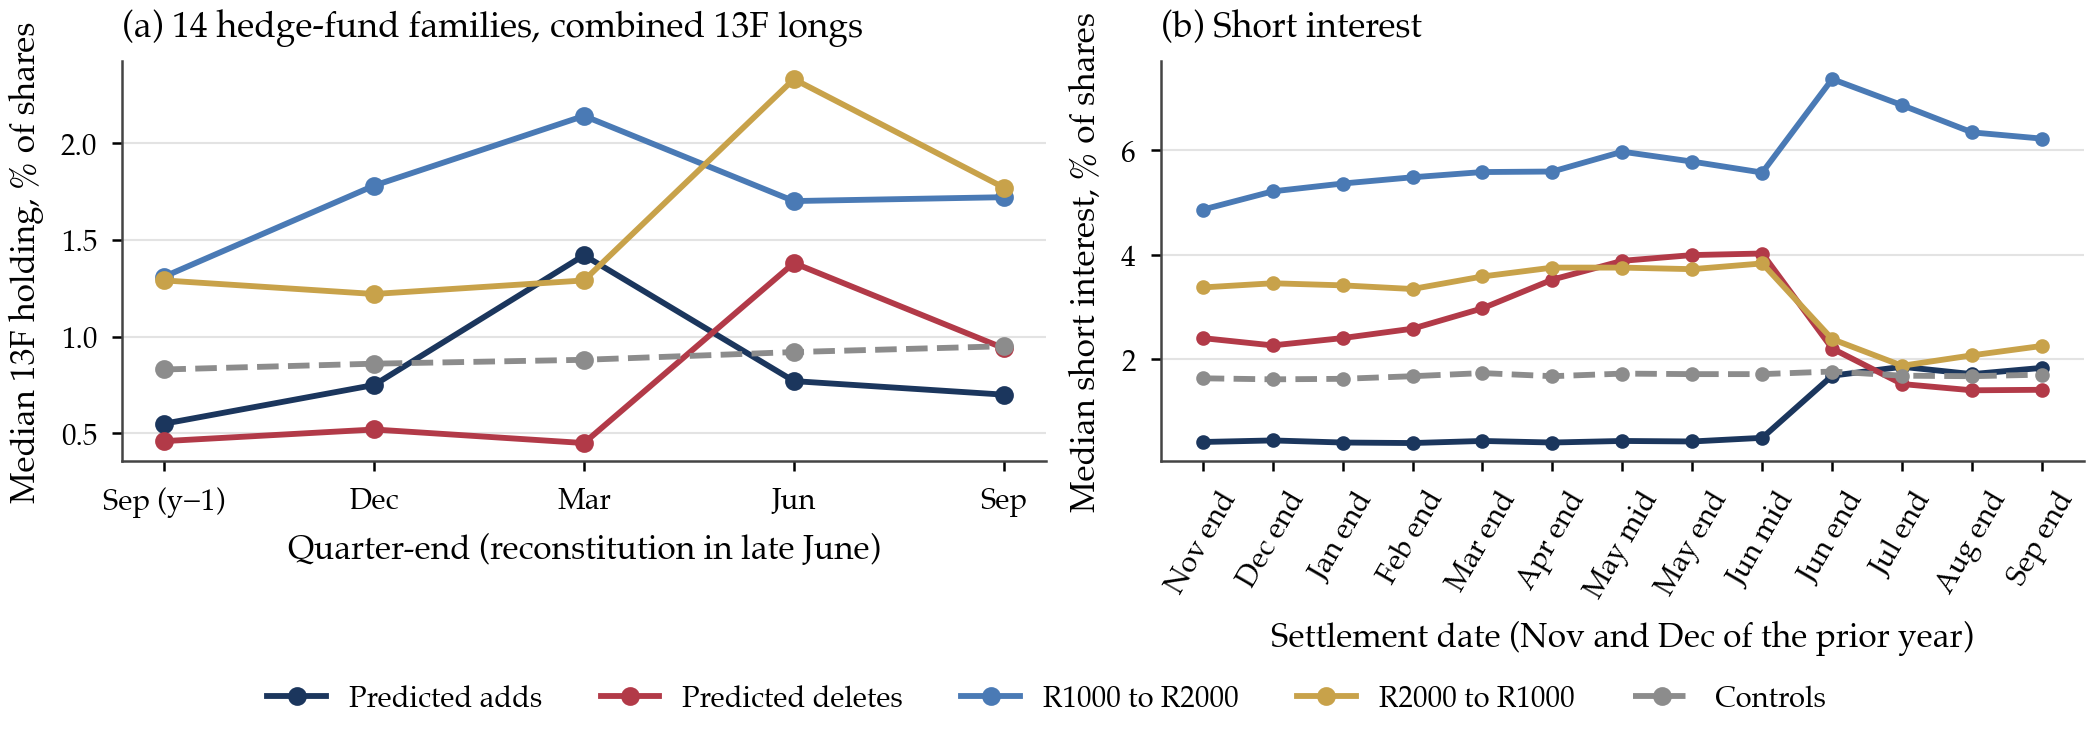
\includegraphics[width=0.92\textwidth]{figures/fig_footprints.png}
\caption{Russell 2016--2025, rank-day-predicted groups: (a) median combined 13F long holdings of fourteen hedge-fund families at the quarter-ends around the June reconstitution; (b) median short interest at each settlement date from November of the prior year to September.}
\label{fig:foot}
\qsource{Thomson Reuters 13F holdings and Compustat short interest via WRDS; author's calculations.}
\end{figure*}

\subsection{The trade-day close and the reversal}

Figure~\ref{fig:closeheat} shows how the close behaves on the trade day for the actual changes, and Figure~\ref{fig:lp} the economics of trading at the close. The close moves reliably with index demand only in US small names and, before 2016, in the DAX family. Russell deletions fell 2.56\% on the trade day ($t = 2.6$, $n = 2{,}783$), but this is a low-price effect: +381 bp below \$5 ($t = 3.2$, $n = 1{,}851$) against +7 bp at \$5 or more ($t = 0.2$). In the one reconstitution for which we have auction prints (27 June 2025), the closing print of sub-\$5 deletions sat 227 bp below the last minute's price, about 37\% of the day's move. Elsewhere the close moves \emph{against} demand: since 2016 S\&P/TSX additions closed 80 bp weak ($t = -2.6$) and deletions 81 bp firm ($t = -2.0$), and STOXX 600 additions closed 43 bp weak ($t = -2.7$), mostly in the UK. This fits a close that is over-supplied by holders who positioned early.

\begin{figure*}[t]
\centering
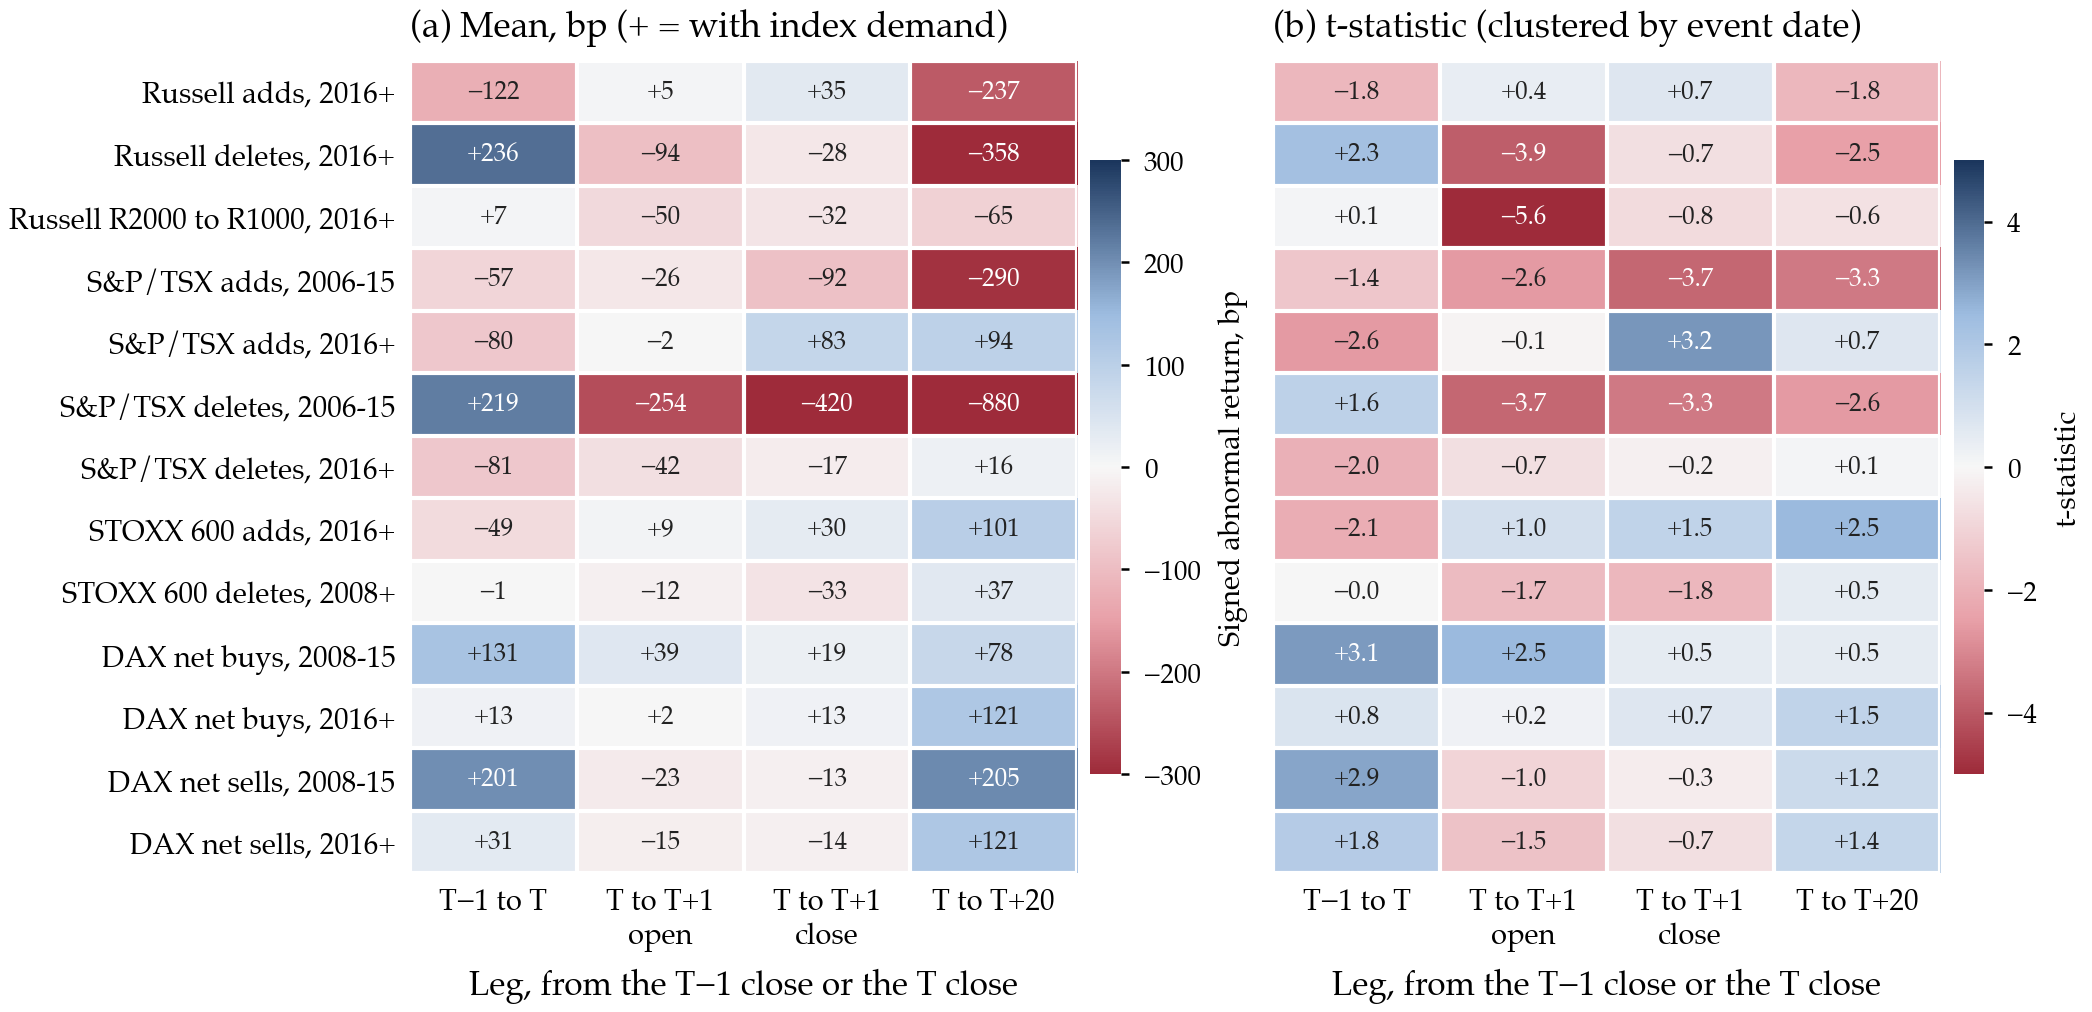
\includegraphics[width=0.92\textwidth]{figures/fig_close_heat.png}
\caption{Trade-day dislocation and reversal for actual index changes by family, side and period: (a) mean signed matched-control abnormal return in bp, positive meaning the price moved in the direction of index demand; (b) t-statistic clustered by event date. Russell June reconstitutions 2008--2025, S\&P/TSX 2006--2026, STOXX 600 2008--2026, DAX family 2008--2025. The T+20 leg sums daily abnormal returns; colours are capped at $\pm$300 bp and $\pm$5.}
\label{fig:closeheat}
\qsource{CRSP, Compustat and Datastream via WRDS; author's calculations.}
\end{figure*}

Where a dislocation exists it reverts mostly overnight. Russell deletions bounced 110 bp by the next open ($t = -3.4$) and then gave some back during T+1. The one liquidity-supply trade that is liquid, consistent across years and holds when hedged with the index is to buy Russell up-migrants (R2000 to R1000), which R2000 trackers sell, at the reconstitution close and sell them at the next open: +42 bp ($t = 4.3$, $n = 578$, 17 of 18 reconstitutions positive), +50 bp since 2016 (10 of 10), +37 bp when hedged with the index rather than controls. These are large names (median capitalisation \$4.7bn), so spreads are a few basis points. In Europe no liquidity-supply trade at the close has paid. The European lead is the opposite trade: buy UK additions \emph{with} the index at the close, +153 bp gross over 20 days ($t = 2.4$), or about 1.0--1.3\% after the 0.5\% UK stamp duty for a buyer that is not exempt. Table~\ref{tab:tax} splits the STOXX 600 by tax regime. The UK pattern is not specific to shares that bear UK stamp duty: foreign-incorporated London lines show the same sign, although only 45 of them exist, so the test has low power.

\begin{figure*}[t]
\centering
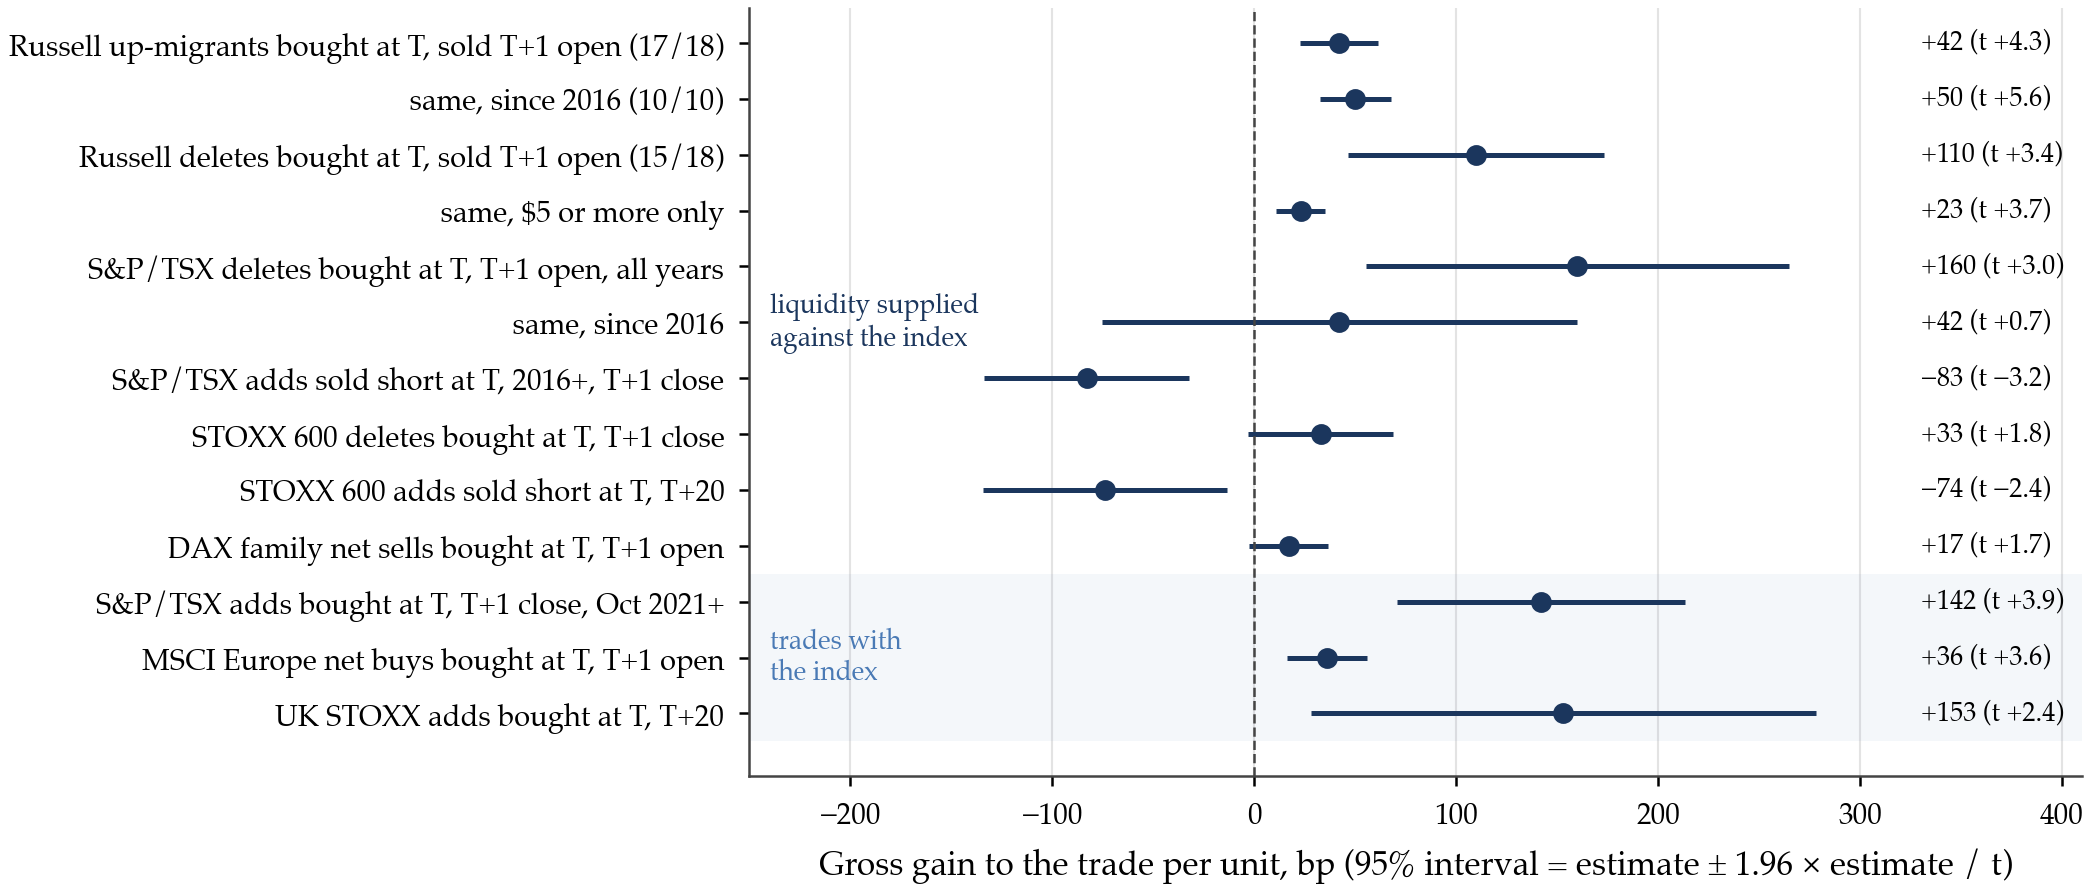
\includegraphics[width=0.92\textwidth]{figures/fig_close_forest.png}
\caption{Trades at the trade-day close: gross gain per unit with 95\% intervals (estimate $\pm$ 1.96 $\times$ estimate/t, t clustered by event date). The upper rows supply liquidity against index demand; the shaded rows trade with it. Event dates positive in brackets where reported. Samples as in Figure~\ref{fig:closeheat}; MSCI Europe 2018--2026; S\&P/TSX since 18 October 2021.}
\label{fig:lp}
\qsource{CRSP, Compustat and Datastream via WRDS; iShares holdings; author's calculations.}
\end{figure*}

\begin{figure}[t]
\centering
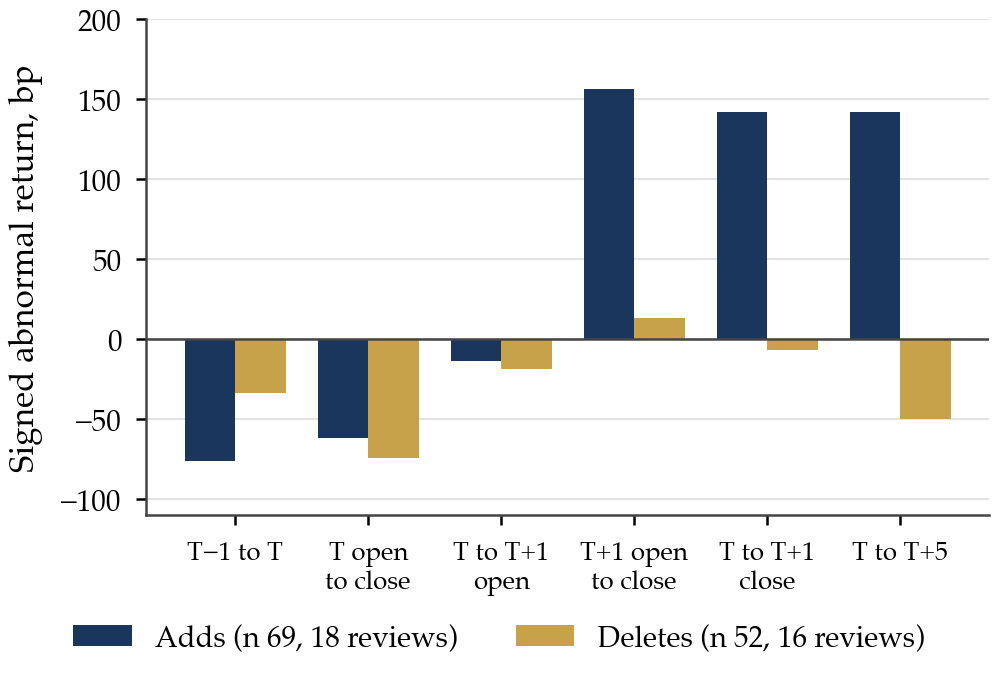
\includegraphics[width=\columnwidth]{figures/fig_tsx_redesign.png}
\caption{S\&P/TSX Composite review changes after the TSX closing redesign (18 October 2021 to June 2026): signed matched-control abnormal return by leg, bp. Positive means a move in the direction of index demand. The T+5 leg sums daily abnormal returns.}
\label{fig:tsxred}
\qsource{Compustat prices and Datastream primary quotes via WRDS; author's calculations.}
\end{figure}

\paragraph{Canada after the 2021 redesign.} Splitting the S\&P/TSX sample at the first close under the new TSX rules (18 October 2021), additions still close weak on the trade day ($-$76 bp, $t = -1.1$) and recover +142 bp by the next close ($t = 3.9$; median +125 bp; 15 of 18 reviews positive; $n = 69$; Figure~\ref{fig:tsxred}). Unlike the US and Europe, the recovery happens during the next session, not overnight. It is not a bid--ask artefact: by spread tercile the rebound is +126, +267 and +32 bp, smallest in the widest-spread names. Deletions show nothing. The sample is small and the two largest review means are recent.

\begin{table}[t]
\centering
\caption{STOXX Europe 600 legs by tax regime of the listing country, signed matched-control bp (t), from the T$-$1 close to the T close, the T+1 open and T+20. Tax start dates are applied, so a French, Italian or Spanish event before its tax counts as untaxed.}
\label{tab:tax}
\footnotesize
\setlength{\tabcolsep}{2.6pt}
\qstripes
\begin{tabularx}{\columnwidth}{@{}Llrrrr@{}}
\toprule
\qhead{Regime} & \qhead{Side} & \qhead{n} & \qhead{T$-$1$\to$T} & \qhead{T+1 open} & \qhead{T+20} \\
\midrule
UK (0.5\%) & add & 194 & \mn132 (\mn3.3) & +48 (2.7) & +153 (2.4) \\
UK & delete & 200 & \mn120 (\mn2.6) & +14 (1.1) & +18 (0.1) \\
FR/IT/ES & add & 66 & +37 (1.2) & +7 (0.5) & +154 (2.1) \\
FR/IT/ES & delete & 65 & +94 (1.7) & +30 (2.1) & +24 (0.2) \\
Untaxed & add & 359 & \mn10 (\mn0.8) & \mn1 (\mn0.1) & +7 (0.2) \\
Untaxed & delete & 354 & +46 (1.6) & \mn31 (\mn2.9) & +47 (0.6) \\
\midrule
\multicolumn{3}{@{}l}{UK $-$ untaxed, pooled} & \mn145 (\mn4.0) & +46 (3.1) & +58 (0.6) \\
\bottomrule
\end{tabularx}
\qsource{Compustat Global, Datastream constituent lists, volume and free float, and Worldscope via WRDS; author's calculations.}
\end{table}

\begin{table}[t]
\centering
\caption{MSCI Canada (CA) and MSCI Europe (EU) review closes: signed matched-control bp (t clustered by review) from the T$-$1 close to the T close, the T+1 open and the T+1 close; Datastream primary-quote prices. ``Oct 21+'' starts at the first close under the new TSX closing rules (18 October 2021); ``to Oct 21'' is 2018 to that date. Net buy or sell is the sign of net visible passive demand.}
\label{tab:msci}
\footnotesize
\setlength{\tabcolsep}{3pt}
\qstripes
\begin{tabularx}{\columnwidth}{@{}lllrRRR@{}}
\toprule
 & \qhead{Net} & \qhead{Sample} & \qhead{n} & \qhead{T$-$1$\to$T} & \qhead{T+1 open} & \qhead{T+1 close} \\
\midrule
CA & buy & Oct 21+ & 14 & \mn13 (\mn0.1) & +35 (1.0) & \mn0 (\mn0.0) \\
CA & sell & to Oct 21 & 21 & +225 (1.7) & \mn10 (\mn0.7) & \mn201 (\mn5.0) \\
CA & sell & Oct 21+ & 17 & +7 (0.1) & +16 (0.7) & \mn52 (\mn0.5) \\
EU & buy & 2018+ & 141 & \mn3 (\mn0.1) & +36 (3.6) & +9 (0.3) \\
EU & buy & Oct 21+ & 77 & \mn2 (\mn0.1) & +41 (2.7) & +46 (1.0) \\
EU & sell & 2018+ & 128 & \mn50 (\mn1.5) & +0 (0.0) & \mn49 (\mn1.7) \\
EU & sell & Oct 21+ & 85 & \mn14 (\mn0.4) & +14 (0.9) & \mn19 (\mn0.6) \\
\bottomrule
\end{tabularx}
\qsource{iShares UCITS holdings; Datastream primary-quote prices via WRDS; author's calculations.}
\end{table}

\paragraph{MSCI review closes.} On MSCI review closes the price does not move with net index demand on the trade day in either market (Table~\ref{tab:msci}). Since the TSX redesign, MSCI Canada net buys moved $-$13 bp ($n = 14$) and net sells +7 bp ($n = 17$), both with $t \approx 0$; MSCI Europe 2018--2026 net buys moved $-$3 bp ($n = 141$) and net sells $-$50 bp ($t = -1.5$, $n = 128$). European net-buy names kept rising overnight: +36 bp to the next open against matched controls ($t = 3.6$) but +24 bp ($t = 2.3$) against the STOXX 600 member index, so the result depends on the benchmark and is suggestive. With 14--17 Canadian events, the Canadian rows cannot exclude a move of the S\&P/TSX size; they say that none is visible. The pre-2021 Canadian sell reversal rests on eight reviews and largely on the May 2020 review.

\subsection{Does bigger flow move the close more?}

\begin{figure}[t]
\centering
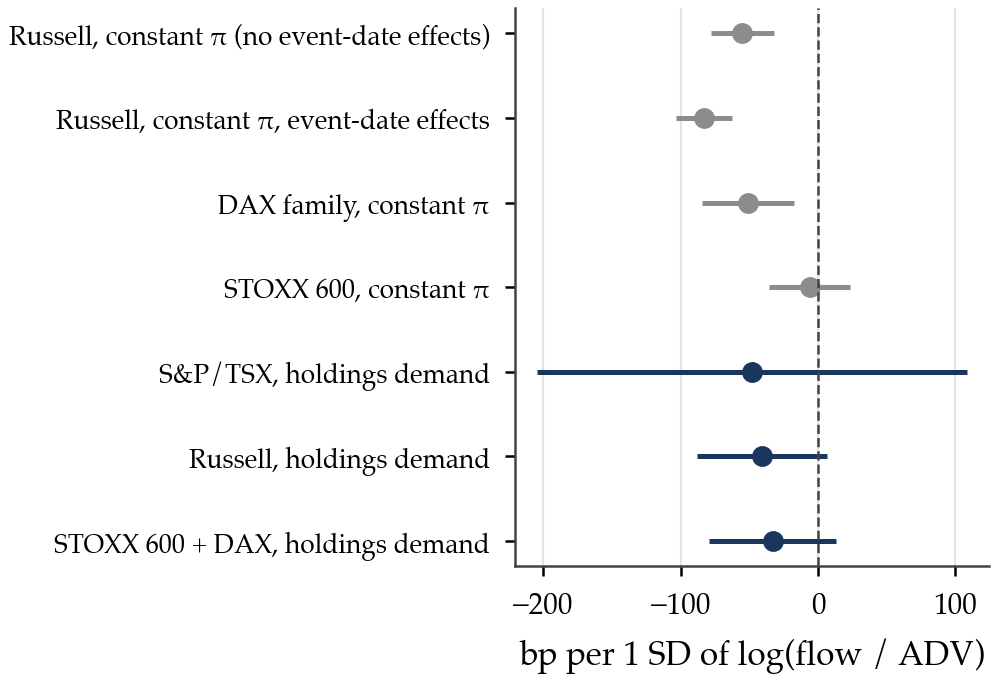
\includegraphics[width=\columnwidth]{figures/fig_flow_forest.png}
\caption{Trade-day move per one standard deviation of log(flow / average daily volume), bp, with 95\% intervals (estimate $\pm$ 1.96 $\times$ estimate/t). Grey: a single passive share per family, which makes flow/volume almost inverse turnover. Navy: holdings-implied demand, with turnover, size, price bucket and event-date fixed effects. Russell 2008--2025; S\&P/TSX 2006--2026; Europe 2008--2026.}
\label{fig:flow}
\qsource{CRSP, Compustat and Datastream via WRDS; iShares and Thomson fund holdings; author's calculations.}
\end{figure}

A first test regressed the trade-day move on predicted flow over average daily volume and found a \emph{negative} coefficient in the Russell and the DAX family. That test is confounded: with a single $\pi$ per family, flow over volume is essentially inverse turnover (correlation $-$0.95 in the Russell). Holdings-implied demand breaks most of that link: its correlation with log turnover falls to $-$0.42 (S\&P/TSX), $-$0.84 (Russell) and $-$0.49 (Europe). With turnover, size, price bucket and event-date fixed effects, one standard deviation more of log true demand over volume moves the close by $-$48 bp in the S\&P/TSX ($t = -0.6$, $n = 618$), $-$41 bp in the Russell ($t = -1.7$, $n = 5{,}951$) and $-$33 bp in the STOXX 600 and DAX family ($t = -1.4$, $n = 705$). None is positive (Figure~\ref{fig:flow}). Weight changes in existing members do not dislocate more when they are larger either. The practical reading is that a desk pricing a closing risk trade should not scale its charge with flow over volume; where flow is largest relative to liquidity, the other side has usually been arranged in advance.

Crowding shows up after the close rather than in it. In the STOXX 600, one standard deviation more run-up into the announcement goes with 44 bp more reversal by the next close ($t = -3.3$), and larger disclosed shorts in deletions with a 33 bp larger next-day rebound ($t = -2.4$). No crowding variable reduces the trade-day move. In Russell deletions, more short interest goes with a \emph{larger} fall on the trade day (+85 bp per standard deviation, $t = 2.3$), the wrong sign for crowded shorts covering into the close.

%═══════════════════════════════════════════════════════
\section{Robustness}
\label{sec:robust}

\paragraph{Early against late.} Figure~\ref{fig:earlylate} puts the main capturable trades side by side for the two halves of each sample. The trades that paid before 2016 (Russell additions from end-December, Russell and S\&P/TSX deletion shorts from the ranking date) do not pay after it. The two that pay after 2016 (S\&P/TSX additions from three months out, DAX-family promotions from six months out) did not pay before it. A result that flips with the period is weaker evidence than one that holds in both; we read the late-period pockets as current but not yet established.

\begin{figure}[t]
\centering
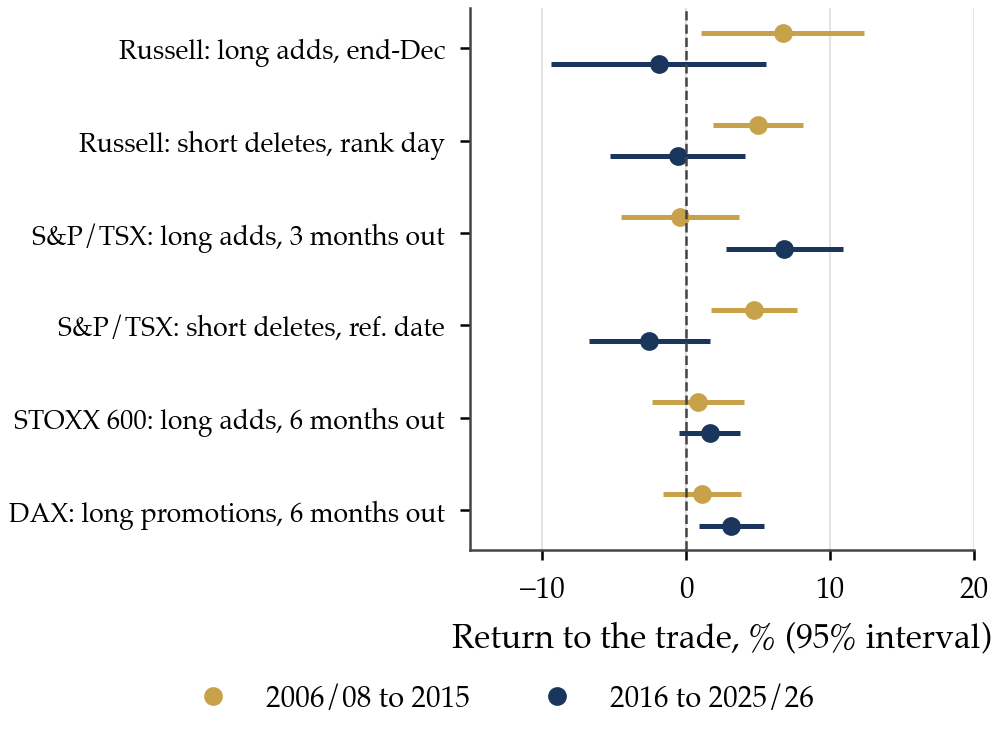
\includegraphics[width=\columnwidth]{figures/fig_early_late.png}
\caption{Headline capturable trades in the early and late halves of each sample, return to the trade with 95\% intervals (estimate $\pm$ 1.96 $\times$ estimate/t). Russell: buy-and-hold, 2008--2015 against 2016--2025; others: CARs, S\&P/TSX 2006--2015 against 2016--2026, STOXX and DAX 2008--2015 against 2016--2026.}
\label{fig:earlylate}
\qsource{CRSP, Compustat and Datastream via WRDS; author's calculations.}
\end{figure}

\paragraph{Year by year.} Figure~\ref{fig:rusyears} shows the Russell long-short spread for each reconstitution. From end-December it was positive in 6 of 8 years before 2016 and 7 of 10 after, but the later years include losses of 14.3\% (2021) and 11.2\% (2024). From rank day the late-period spread was negative in 5 of 10 years. Ten clusters after 2016 leave few results above $|t| = 2$.

\begin{figure*}[t]
\centering
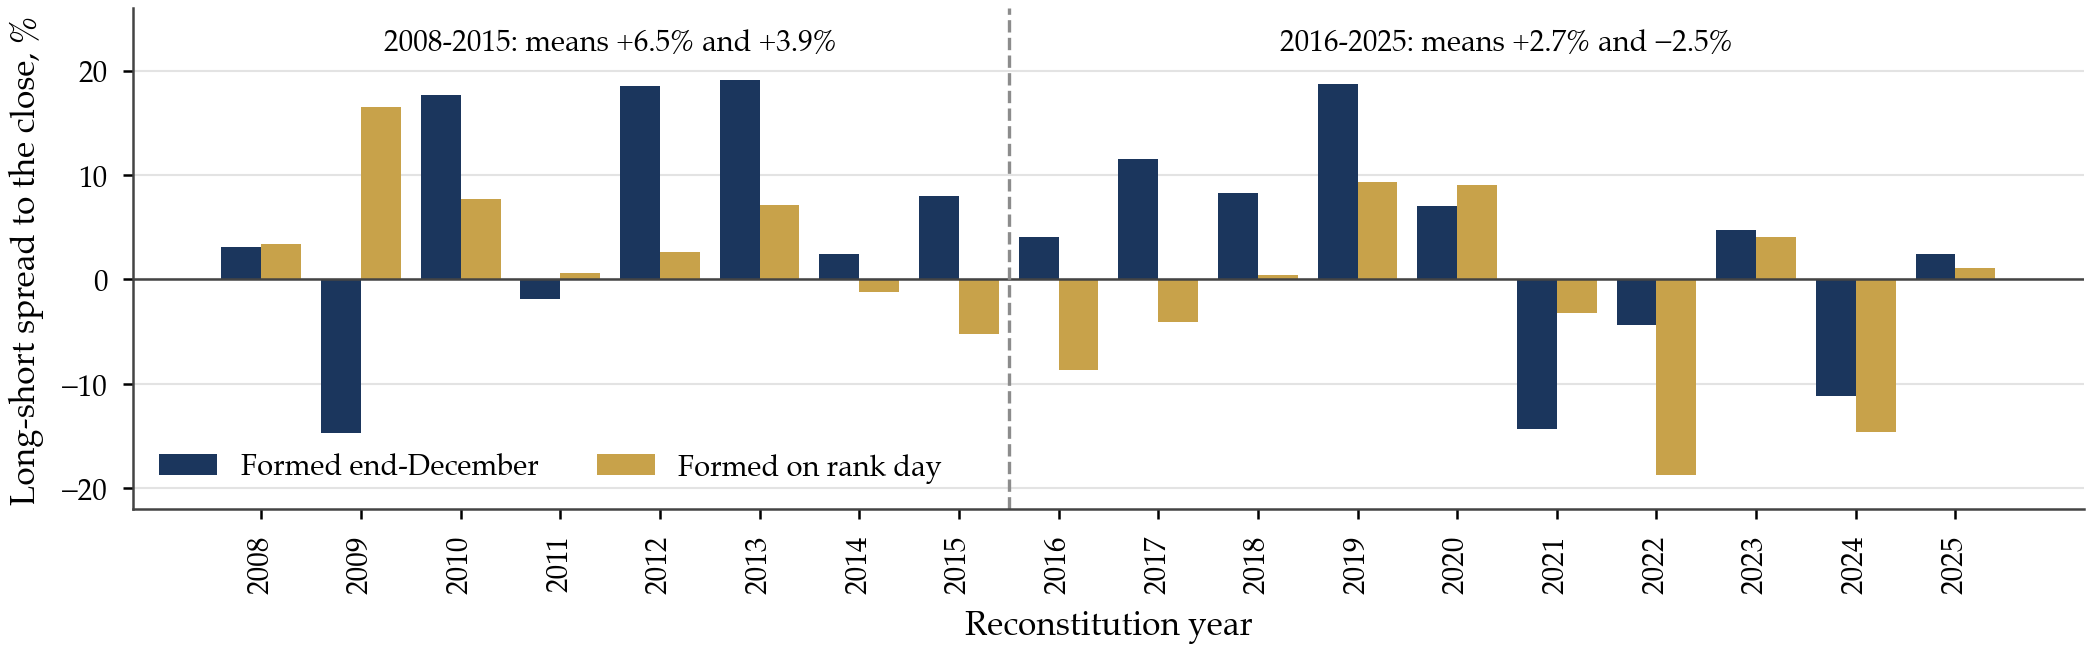
\includegraphics[width=0.92\textwidth]{figures/fig_russell_years.png}
\caption{Russell equal-weighted long predicted additions / short predicted deletions, abnormal spread per reconstitution to the reconstitution close, 2008--2025, for portfolios formed at end-December and on rank day.}
\label{fig:rusyears}
\qsource{CRSP and Datastream Russell constituent lists via WRDS; author's calculations.}
\end{figure*}

\paragraph{Means, medians and outliers.} The STOXX six-month addition result is the case where outliers matter: eight names whose summed abnormal return fell below $-$100\% pull the mean to +1.3\% ($t = 1.4$); the median is +2.0\%, the 10\% trimmed mean +2.2\% and the mean with each name floored at $-$100\% is +1.7\% ($t = 1.9$). Even the most favourable reading stops short of $t = 2$. The DAX six-month promotion result is stable across these choices (median +2.4\%, floored +2.2\%, $t = 2.4$). Dropping the best review leaves STOXX six-month additions at +1.1\% ($t = 1.2$) and DAX promotions at +2.0\% ($t = 2.2$).

\paragraph{Post-hoc choices.} Without the STOXX eligibility proxies, predicted additions return $-$0.55\% from three months out ($t = -1.3$) and $-$0.25\% from the cut-off, so the STOXX conclusion does not depend on them. For the S\&P/TSX the plain rules give +3.4\% rather than +6.8\%; we treat the lower figure as the estimate.

\paragraph{Benchmarks.} Against cap-weighted index proxies instead of matched controls, the signs and conclusions hold: S\&P/TSX three-month additions +2.4\% ($t = 1.5$) over the full sample, STOXX six-month additions +1.7\% ($t = 1.3$), DAX six-month promotions +1.6\% ($t = 1.6$). For Russell additions on the trade day the benchmark matters: $-$87 bp against controls but $-$14 bp against the Russell 2000 ETF, because small-cap controls rose on reconstitution days.

\paragraph{Checks and corrections.} Every headline number in the European study was recomputed from the event-level files. This found and fixed four problems: a one-month gap in the Datastream TecDAX list (August 2017) that had created 28 false promotions; a recall denominator that left out actual moves the screen never ranked; a look-ahead in the naive STOXX benchmark; and summed abnormal returns below $-$100\% in the capacity arithmetic. In the close study, 180 headline cells were recomputed with independent code (maximum difference $3\times10^{-13}$ bp), and dropping opens equal to the previous close moved every overnight mean by 10 bp or less.

%═══════════════════════════════════════════════════════
\section{Capacity and implementation}
\label{sec:capacity}

Table~\ref{tab:cap} gives deployable size and gross P\&L per event at 10\% participation. The numbers are small for a single trade. The S\&P/TSX three-month addition trade takes a median of about C\$113m per review across three names; the DAX six-month promotion trade about \texteuro860m across 11.5 names, but weighted by what can be deployed it earns $-$0.3\%, because the liquid names do not earn the return. The Russell deletion short trades names with median daily value traded of \$0.85m and quoted spreads of 44--50 bp. Liquidity supply at the close is smaller still outside the US: at 10\% of visible demand it is about C\$6m in additions and C\$2m in deletions per S\&P/TSX review and \texteuro3--6m per side per STOXX or DAX review. Visible demand understates the true close several times (Table~\ref{tab:demand}), so these are conservative.

\begin{table*}[t]
\centering
\caption{Capacity at 10\% participation and gross P\&L per event at the measured mean return, before spreads, impact, taxes and borrow. The arithmetic assumes the full position is in place at formation; building it over the window earns less.}
\label{tab:cap}
\footnotesize
\qstripes
\begin{tabularx}{\textwidth}{@{}LP{3.5cm}P{3.6cm}P{5.0cm}@{}}
\toprule
\qhead{Trade} & \qhead{Deployable per event} & \qhead{Gross P\&L per event} & \qhead{Comment} \\
\midrule
Russell: short predicted deletes from end-Dec (2016--25) & \$309m per recon & \$7.5m at the equal-weighted mean & 156 names; median ADV \$0.85m; quoted spread 44 bp; borrow unknown \\
Russell: buy up-migrants at the close, sell next open & \$405m (\$503m since 2016) & \$2.2m (\$3.1m) & 10\% of predicted R2000-tracker selling \\
S\&P/TSX: predicted adds from H3 (2021--26) & C\$113m per review (C\$33m per name) & C\$2.2m at +2.0\%; C\$7.7m at +6.8\% & Median ADV C\$5.3m, 63.5 sessions, 3 names \\
S\&P/TSX: buy adds at the close, sell next close (since Oct 2021) & About C\$16m per review & About C\$0.2m at +142 bp & 5\% of trade-day volume, about 4 adds; a pricing input more than a strategy \\
DAX family: predicted promotions from H6 (2021--26) & \texteuro860m per review (\texteuro30m per name) & \texteuro27m at +3.2\%; $-$\texteuro2.7m deploy-weighted & 11.5 names; the liquid names do not earn the return \\
STOXX 600: predicted adds from H6 (2021--26) & \texteuro1.28bn per review & \texteuro22m at +1.7\% (not significant) & 16 names; median ADV \texteuro5.6m \\
\bottomrule
\end{tabularx}
\qsource{CRSP, Compustat and Datastream volume via WRDS; author's calculations.}
\end{table*}

\paragraph{Costs not modelled.} Every return in this paper is gross. The main costs are known in outline. Russell deletion names quote a median spread of 44--50 bp. S\&P/TSX additions since 2021 have a median closing quoted spread of 132 bp on the trade day and 98 bp the day after, from end-of-day quotes that probably overstate the spread during the session; a trade done in the closing auction at both ends crosses no spread but pays auction fees and impact. Buys in the UK, Ireland, France, Italy and Spain carry a transaction tax (0.5\% stamp duty in the UK, 1\% in Ireland, 0.4\% in France since April 2025, 0.2\% in Italy and Spain). Indicative borrow fees for 48 S\&P/TSX and STOXX names around the 2025--26 trade days were about 1\% a year with no spike around the event (median 1.36\% for S\&P/TSX additions and 0.86--0.90\% for STOXX deletions); that is immaterial for a one- to five-day trade but not for 20-day holds in small names, and the costly cases (US sub-\$5 names) are not covered.

\paragraph{Hedging with index futures.} A desk that hedges a closing basket with index futures is exposed when the future settles before the cash closing auction. Eurex (EURO STOXX 50, STOXX 600, DAX, SMI), ICE (FTSE 100 and 250) and MEFF (IBEX 35) futures settle before the cash close; on normal days the cash index then moves a median 6--9 bp in the auction. On quarterly expiry Fridays the standard deviation of that move is 16--23 bp and on MSCI review closes 17--26 bp, 1.2--1.7 times normal. For a \texteuro1bn basket with beta one that is about \texteuro1.6--2.6m at one standard deviation. Euronext CAC 40 and AEX futures, FTSE MIB futures since 2024 and the mini S\&P/TSX Composite future settle on the close and avoid it. At quarter-ends that are not expiry days the European cash auction moved $-$4.9 bp on average ($t = -2.6$; $-$7.3 bp since 2018).

%═══════════════════════════════════════════════════════
\section{Forward paper tests on 2026 reviews}
\label{sec:forward}

The historical studies were followed by paper forecasts of the 2026 reviews, made from public data only (provider lists and notices, iShares holdings, exchange directories and free price data). Each forecast run writes its outputs with SHA-256 file hashes into an append-only log before the outcome is known, and a run that would overwrite an earlier one moves the old file aside. These are simulated forecasts scored, or to be scored, against the actual announcements; no orders were placed. Table~\ref{tab:forward} lists what has been scored so far. All of these are calibration replays or backfills of reviews that had already happened when the code was written, so they are not out of sample, and several carry look-ahead in the inputs (for example, today's share counts).

\begin{table*}[t]
\centering
\caption{Paper forecasts scored against 2026 announcements (replays and backfills, not out of sample). Precision / recall, \%.}
\label{tab:forward}
\footnotesize
\qstripes
\begin{tabularx}{\textwidth}{@{}P{3.4cm}P{3.3cm}L@{}}
\toprule
\qhead{Review} & \qhead{Type} & \qhead{Result} \\
\midrule
Russell, June 2026 & Rank-day rebuild with current share counts (look-ahead) & R3000 additions 59 / 83 (184 hits of 313 predicted; 221 actual); deletions 74 / 92 (104 of 141; 113 actual). The rebuilt rank-3,000 cut-off was \$187m against FTSE Russell's published \$146.4m. \\
S\&P/TSX, June 2026 & Backfill at the reference date & Rules: additions 5 of 7 (71 / 100), deletions 5 of 5. Main model: additions 4 of 4 (100 / 80). Paper return to the trade close: rules additions +1.79\% against the iShares XIC index ETF, main +3.73\%, short deletions $-$1.26\%. \\
S\&P/TSX, September 2026 & Backfill at the reference date & Rules: 1 of 3 additions (33 / 100); main model predicted none. Rules additions $-$5.17\% against XIC. The committee-memory filter wrongly dropped the one actual addition in each of June and September. \\
MSCI, May 2026 & Replay (pseudo point in time) & With a 1.07 cut-off drift factor: Europe deletions 8 of 9 found, all 8 calls correct; Canada 1 of 1; none of 4 additions found. Without the drift factor: Europe deletions 4 of 9. The drift factor was chosen on this replay. \\
STOXX 600, June 2026 & Replay & At the cut-off: additions 12 of 14 (86 / 100), deletions 8 of 12 (67 / 80). Seven weeks out: additions 2 of 4 (50 / 17), no deletions predicted (10 actual). \\
DAX family, June 2026 & Replay & At the cut-off: 12 of 14 moves (86 / 60). Seven weeks out: 3 of 6 (50 / 15). \\
FTSE 100/250, June 2026 & Replay & At the cut-off: 9 of 18 (50 / 50); with point-in-time Datastream capitalisations 9 of 14 (64 / 50). Seven weeks out: 4 of 14 (29 / 22). \\
\bottomrule
\end{tabularx}
\qsource{provider lists and notices, iShares holdings files, exchange directories and public price data; author's calculations.}
\end{table*}

\begin{figure}[t]
\centering
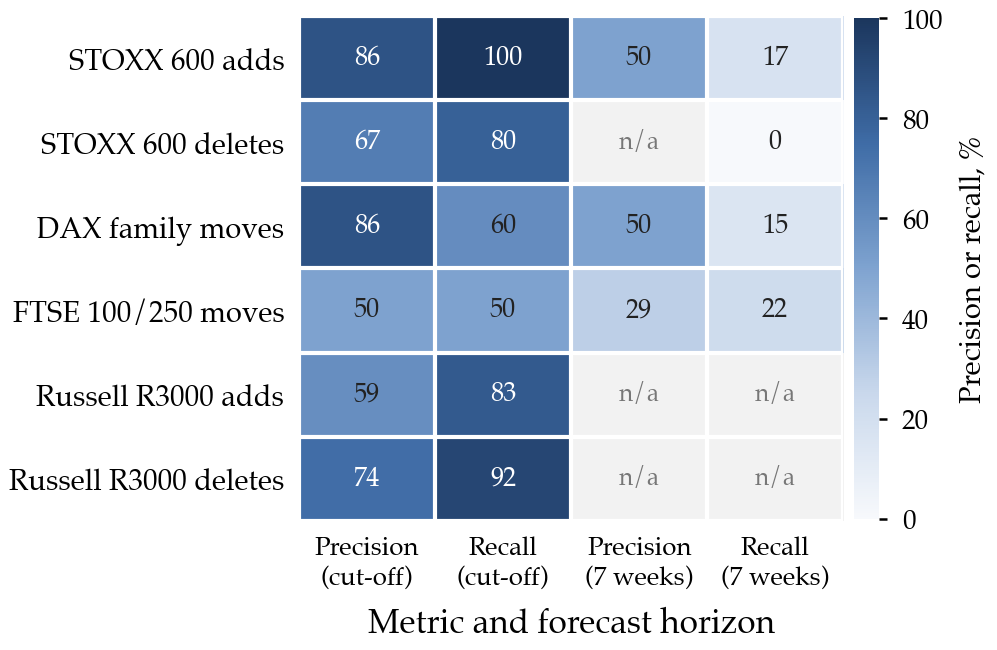
\includegraphics[width=\columnwidth]{figures/fig_forward.png}
\caption{June 2026 calibration replays of the free-data forecasts: precision and recall at the ranking cut-off and seven weeks before it, \%. Russell rows are rank-day rebuilds with current share counts; ``n/a'' marks a horizon not run or with no predictions. Replays, not out-of-sample tests.}
\label{fig:forward}
\qsource{provider lists and notices, iShares holdings files and public price data; author's calculations.}
\end{figure}

The replays say the same thing as the historical studies (Figure~\ref{fig:forward}): free-data rebuilds are accurate at the ranking date and much weaker weeks before it. Seven weeks out, the June 2026 STOXX replay found 2 of 12 additions and none of 10 deletions.

\paragraph{Logged forecasts awaiting scoring.} Out-of-sample forecasts were logged in October 2026 for the November MSCI review (trade close 30 November) and the December Russell, S\&P/TSX, STOXX 600, DAX-family and FTSE UK reviews (11 and 18 December). The Russell run on the 9 October close predicted 98 new R2000 additions, 66 deletions and 16 migrations between the R1000 and R2000. The S\&P/TSX run on the same close, about ten weeks before the trade, predicted three additions and two deletions under the plain rules and one addition and two deletions under the main model. The MSCI run implied about 4.3 expected changes in MSCI Canada and 13.0 in MSCI Europe (sums of probabilities); its first version was corrected on 13 October, before any outcome, and the log records why. The European run on the 12 October close implied about 16 expected STOXX 600 changes, no near-certain DAX-family move, and four deterministic FTSE 100/250 calls. These forecasts are re-run at each ranking date and scored after the announcements; the results were not available when this paper was written and are not reported here.

\paragraph{Demand engine.} The same forecasts feed a net-flow engine that adds up, per stock, the demand from every index trading the same close, using Equation~\eqref{eq:demand} with the measured $R$. On the 19 June 2026 close, with the actual index changes as inputs (which a desk would have from provider files), predicted demand ranked abnormal trade-day volume well for additions and deletions (Spearman 0.82, $n = 58$; $R^2$ of log on log 0.87) and poorly for share, float and capping updates (0.35, $n = 230$). On the 26 June 2026 Russell close the rank correlation was 0.72 ($n = 341$). This validates the sizing of the flow, not the forecast of which names change; that test needs the December events.

%═══════════════════════════════════════════════════════
\section{Limitations and open questions}
\label{sec:limits}

\textbf{Gross returns.} No spreads, market impact, borrow fees or transaction taxes are deducted anywhere, and fills are assumed at the official close and open. Deletion shorts in small names may have been expensive or impossible to borrow; we have no historical borrow data.

\textbf{Point in time, but not perfectly.} Membership is exact and survivorship-free, but Compustat headquarters, domicile, industry and security type are current values applied to history; CRSP and Datastream share and float histories may be restated; and controls exclude names that actually changed, which uses hindsight. The provider rules come from 2025--2026 editions and are applied backward; DAX-family thresholds before 2021 are inferred, and S\&P/TSX announcement dates before 2019 and some Russell rank-day and preliminary-list dates are reconstructed. The horizon-to-close, trade-day and post-event windows do not depend on the announcement date.

\textbf{Small samples and many tests.} There are 10 Russell reconstitutions since 2016, 102--181 S\&P/TSX three-month additions since 2016, 69 S\&P/TSX additions since the 2021 redesign and 14--17 MSCI Canada events since then. Many windows, sides, eras and variants were tested, which is why $|t| < 2.5$ is read as suggestive.

\textbf{Measurement.} Volume bases differ (TSX-only against consolidated, primary venue against all lit venues) and change multiples by 1.2--2 times. European volume is mostly primary venue, so European $R$ is a lower bound. Same-day index events (FTSE UK, Euronext, SMI and others on the same third Friday) are not removed from the controls. The 13F holdings are long-only, quarterly and filed with a lag, and the funds tracked run many strategies, so the footprints are descriptive.

\textbf{Open questions.} The most important open questions are the share of TSX volume in the closing auction on index days and the path of the auction imbalance; how fast closing dislocations revert outside the US; the cost of borrowing deletion candidates between announcement and trade in Canada and Europe; the cost of trading in Canadian and European closing auctions; and how often providers delete the same takeover target on different dates. Each needs data we do not yet have: auction imbalance feeds, securities-lending data and intraday European prices.

%═══════════════════════════════════════════════════════
\section{Conclusion}
\label{sec:conclusion}

Index funds still have to trade at the close, and the flow is large: on the trade day, changing names trade several times their normal volume, and the volume-implied passive share is several times the share held by visible ETFs. But the money from that obligation is not where announcement-window studies look for it, and most of it is not capturable by a rules replication on public data. The large moves in names that change are selection. The broad trade of holding predicted changes into the close paid before 2016 and has not paid since in the Russell or the S\&P/TSX, and it never paid reliably in the STOXX 600. Holdings data show traders building positions months ahead and supplying the close, which is consistent with the edge having moved into the prediction window and into the hands of those with better rule inputs.

What remains, gross of costs, is narrow and small: S\&P/TSX additions predicted three months out (+3.4\% under the plain rules), small-cap DAX-family promotions, the 20-day rebound of Russell deletions, an overnight liquidity-supply trade in Russell up-migrants worth about \$2--3m per reconstitution, and a next-session rebound in S\&P/TSX additions since 2021 on 69 events. None has yet been tested net of measured costs. The logged forecasts for the November and December 2026 reviews are the first out-of-sample test of the prediction step.

%═══════════════════════════════════════════════════════
\section*{Code availability}

{\raggedright
The scripts for every study are in this repository under \texttt{code/index\_rebalance\_research/}: the event studies under \texttt{12\_studies/} (\texttt{russell\_june/}, \texttt{tsx\_composite/}, \texttt{stoxx600\_dax/}, \texttt{close\_dislocation/}, \texttt{net\_flow/}, \texttt{msci\_pi/}, \texttt{msci\_close/}, \texttt{expiry\_basis/}), the forward paper forecasts under \texttt{13\_shadow/}, the borrow-fee collection under \texttt{14\_borrow\_data/}, the net-flow engine under \texttt{16\_flow\_engine/} and the methodology refresh tools under \texttt{11\_methodology/tools/}. The data are licensed (CRSP, Compustat, Refinitiv Datastream and Worldscope, Thomson Reuters 13F and SDC, accessed through WRDS) or cached from public sources, and are not distributed.\par}

%═══════════════════════════════════════════════════════
\begin{thebibliography}{99}
\small

\bibitem{greenwood2025}
Greenwood and Sammon.
\newblock ``The Disappearing Index Effect.''
\newblock \textit{Journal of Finance}, 80(2):657--698, 2025. NBER Working Paper 30748, 2022.

\bibitem{chinco2024}
Chinco and Sammon.
\newblock ``The Passive-Ownership Share Is Double What You Think It Is.''
\newblock \textit{Journal of Financial Economics}, 157, 103860, 2024.

\bibitem{petajisto2011}
Petajisto.
\newblock ``The index premium and its hidden cost for index funds.''
\newblock \textit{Journal of Empirical Finance}, 18(2):271--288, 2011.

\bibitem{dfa2024}
Hendrix, Liu and Roberts (Dimensional Fund Advisors).
\newblock ``Measuring the costs of index reconstitution: a 10-year perspective.''
\newblock Dimensional, July 2024.

\bibitem{dfa2025}
Hendrix, Liu and Roberts (Dimensional Fund Advisors).
\newblock ``Measuring the costs of index reconstitution: evidence outside the US.''
\newblock Dimensional, January 2025.

\bibitem{bm2023}
Bogousslavsky and Muravyev.
\newblock ``Who trades at the close? Implications for price discovery and liquidity.''
\newblock \textit{Journal of Financial Markets}, 66, 100852, 2023.

\bibitem{spdji}
S\&P Dow Jones Indices.
\newblock \textit{S\&P/TSX Canadian Indices Methodology.} June 2025 edition.

\bibitem{stoxx}
STOXX Ltd.
\newblock \textit{STOXX Index Methodology Guide} and \textit{STOXX Calculation Guide.} September 2026 editions.

\bibitem{dax}
STOXX Ltd.\ (Deutsche B\"orse group).
\newblock \textit{DAX Equity Index Methodology Guide}, version 12.7.3. August 2026.

\bibitem{msci}
MSCI.
\newblock \textit{MSCI Global Investable Market Indexes Methodology.} August 2026.

\bibitem{russell}
FTSE Russell.
\newblock \textit{Russell US Equity Indexes Construction and Methodology}, version 7.2. August 2026.

\end{thebibliography}

\end{document}
